% ============================================================
%  DigiRadio — Technical Manual (main file)
%
%  Compile with LuaLaTeX or XeLaTeX for the real Optima font
%  (a system font on macOS):
%      latexmk -lualatex manual.tex
%  pdfLaTeX also works and falls back to Linux Biolinum.
% ============================================================
\documentclass[12pt,a4paper,oneside]{scrreprt}

\usepackage{digiradio-manual}
\usepackage{tikz}
\usetikzlibrary{positioning, arrows.meta, fit, backgrounds}

\begin{document}

% ---------------- Cover ----------------
\begin{titlepage}
\thispagestyle{empty}
\vspace*{3.5cm}
{\color{drPetrol}\fontsize{48}{52}\selectfont\bfseries DigiRadio\par}
\vspace{3mm}
{\color{drAmber}\rule{\linewidth}{2.5pt}}
\vspace{6mm}

{\color{drInk}\LARGE Open-Source Hi-Fi DAB+/FM Receiver\par}
\vspace{3mm}
{\color{drGray}\Large Technical Manual\par}

\vfill
{\color{drInk}\large Michele Bigi\par}
\vspace{2mm}
{\color{drGray}Firmware 0.9.0 \quad\textbullet\quad 2026\par}
\vspace{2mm}
{\color{drGray}Hardware: CERN-OHL-S v2 \quad\textbullet\quad Firmware: Apache-2.0\par}
\vspace{2mm}
{\color{drGray}\small \url{https://github.com/manvalan/DigiRadio}\par}
\end{titlepage}

% ---------------- Contents ----------------
\pagestyle{plain}
{\color{drPetrol}\tableofcontents}
\clearpage

% ---------------- Chapters ----------------
\chapter{Introduction}
\label{ch:introduction}

DigiRadio is an open-source, high-fidelity digital radio receiver. It
receives DAB+ and FM broadcasts, processes the audio through a dedicated
signal processor, and streams the result over Bluetooth using a
high-resolution codec. Firmware~0.8.3 on \texttt{main} provides encrypted
storage, a tabbed configuration web UI, and the full REST API documented
in Chapter~\ref{ch:api}. The whole project --- hardware and firmware --- is
released as open source for the maker and audio community to study,
build, and improve.

\section{What DigiRadio is}

Most DAB+/FM hobby projects stop at basic reception. DigiRadio adds two
things that lift it into hi-fi territory: a real audio DSP stage for
equalisation and mixing, and a premium-codec Bluetooth output. The result
is a genuine wireless audio source rather than a bench demo, and, being
fully documented, a practical reference for anyone learning multi-chip
audio design or RF-aware PCB layout.

\begin{drkey}[At a glance]
A four-chip design --- Si4684 tuner, ADAU1701 DSP, ESP32-S3 host, and an
FSC-BT1035 Bluetooth transmitter --- on a six-layer board, powered from
USB-C, configured through an elegant web interface.
\end{drkey}

\section{Who this manual is for}

This manual documents the system for someone building, flashing, or
extending DigiRadio: the hardware at a block level
(Chapter~\ref{ch:hardware}), the firmware architecture
(Chapter~\ref{ch:firmware}), dedicated companion-chip guides for the
Si4684 tuner (Chapter~\ref{ch:si4684}) and ADAU1701 DSP
(Chapter~\ref{ch:adau1701}), FSC-BT1035 Bluetooth
(Chapter~\ref{ch:bt1035}), the HTTP JSON API exposed by the web UI
(Chapter~\ref{ch:api}), the per-class design reference that grows with
the code (Chapter~\ref{ch:classes}), and how to build and flash
(Chapter~\ref{ch:build}). Exact C++ signatures are generated by Doxygen
from the source; this manual explains design, behaviour, and the
reasoning behind it.

\section{Licensing summary}

The hardware is licensed under CERN-OHL-S v2 and the firmware under
Apache-2.0; full details are in Chapter~\ref{ch:licensing}. The project
repository is at \url{https://github.com/manvalan/DigiRadio}.

\chapter{Hardware Overview}
\label{ch:hardware}

This chapter describes the board at a block level. The complete hardware
design --- schematics, PCB, Gerbers, and bill of materials --- is
published in the repository under the CERN-OHL-S v2 licence.

\section{System block diagram}

DigiRadio is built around four devices coordinated by the ESP32-S3. The
tuner produces the audio stream, the DSP conditions and mixes it, and the
Bluetooth module transmits it; the host manages all three and provides
the network interface.

\begin{table}[htbp]
  \centering
  \begin{tabular}{@{}lll@{}}
    \drhead Device & Role & Interface \\
    \midrule
    Si4684            & DAB+/FM tuner              & SPI / I\textsuperscript{2}C \\
    ADAU1701          & Audio DSP (EQ + mixer)     & I\textsuperscript{2}C \\
    ESP32-S3-WROOM-1  & Host controller, Wi-Fi/BLE & ---            \\
    FSC-BT1035         & Bluetooth 5.2 (aptX Adaptive) & UART (AT)  \\
    \bottomrule
  \end{tabular}
  \caption{Principal integrated circuits and their roles.}
  \label{tab:hw-ics}
\end{table}

\section{Power}

The board is powered from USB-C. An AP63203 buck converter generates the
main rails from the USB input, feeding the digital and analogue sections.
The tuner's sensitive supplies are derived and filtered separately to
keep RF performance clean.

\section{RF and antennas}

Two 2.4\,GHz radios are present --- the ESP32-S3 and the Bluetooth module.
Their antennas are placed on opposite diagonal corners of the board to
maximise separation and minimise mutual desense. Each module keeps its
antenna keep-out clear of copper on all layers.

\begin{drnote}[Board]
The PCB is a six-layer stack-up with controlled impedance on the USB and
RF sections. The full fabrication data is in the repository.
\end{drnote}

\section{User interface and connectors}

Configuration is done over Wi-Fi through a built-in web interface (see
Chapter~\ref{ch:firmware}); no display is required on the board itself.
Audio reaches the listener wirelessly over Bluetooth.

\chapter{DSP Configuration (SigmaStudio)}
\label{ch:sigmastudio}

This chapter documents how the ADAU1701 is configured in SigmaStudio: the
hardware settings that must match the board, the audio signal-processing
chain, and the parameters exposed for runtime control by the ESP32. The
resulting SigmaStudio export is what the host writes into the DSP's RAM at
every boot (Section~\ref{sec:hw-adau}). For the firmware driver, safeload
API, persistence, and HTTP usage, see Chapter~\ref{ch:adau1701}.

\section{Overview}
\label{sec:ss-overview}

The DSP program is built once in SigmaStudio and exported as a sequence of
register writes. Because the board carries no self-boot EEPROM, the ESP32
replays that sequence over I\textsuperscript{2}C (address 0x34) on every
power-up. SigmaStudio is therefore used purely to \emph{design and export}
the program, not to drive the chip in operation.

\begin{drkey}[No hardware required to export]
The whole program can be built and exported offline, without a physical
ADAU1701 or a USBi programmer connected. A USBi block is placed in the
Hardware Configuration only because SigmaStudio requires a communication
channel to compile.
\end{drkey}

\begin{drref}[Live connection is also possible]
Since firmware~0.9.0, DigiRadio's \texttt{net::SigmaStudioTcpServer}
(Chapter~\ref{ch:adau1701}, Section~\ref{sec:adau1701-sigmastudio-tcp})
exposes a TCP:8086 bridge so SigmaStudio can \emph{Connect} and
\emph{Link Compile Download} directly against a running board, for live DSP
tuning and bench debugging. The export-only workflow below remains the
simplest path for ordinary firmware builds.
\end{drref}

\section{Hardware Configuration}
\label{sec:ss-hwcfg}

The Hardware Configuration tab must mirror the board exactly. The key
settings are collected in Table~\ref{tab:ss-hwcfg}. The 48\,kHz system
sample rate follows from the \textbf{board strapping}, not from a
SigmaStudio preference alone: X1 is a 12.288\,MHz crystal, PLL\_MODE selects
256\,$\times$\,f\textsubscript{S}, and 12.288\,MHz\,/\,256 = 48\,kHz.

\begin{table}[htbp]
  \centering
  \begin{tabular}{@{}L{4.2cm}L{9.2cm}@{}}
    \drhead Setting & Value \\
    \midrule
    Control port (I\textsuperscript{2}C address) & 0x34 (ADDR0/ADDR1 = GND) \\
    Self-boot                     & Disabled (host RAM load) \\
    System sample rate            & 48\,kHz (256\,$\times$\,f\textsubscript{S} strapping) \\
    MCLK                          & 12.288\,MHz crystal (256\,$\times$\,f\textsubscript{S}) \\
    Serial Input format           & I\textsuperscript{2}S, 24-bit \\
    Serial Output                 & \textbf{Master Mode} (ADAU generates clocks) \\
    Word length                   & 24 bits \\
    RAM Modulo / Program Length   & 1x (1024 instructions) \\
    \bottomrule
  \end{tabular}
  \caption{ADAU1701 hardware settings in SigmaStudio.}
  \label{tab:ss-hwcfg}
\end{table}

\begin{drnote}[Clock source on the board]
SigmaStudio's 48\,kHz sample-rate field must agree with the fabricated
hardware: passive crystal X1 (12.288\,MHz, CL = 12\,pF) on MCLKI/OSCO with
22\,pF load caps, PLL\_MODE0 = GND and PLL\_MODE1 = 3V3 (256\,$\times$\,f\textsubscript{S}).
The ADAU1701 internal oscillator multiplies the crystal; it is not an active
oscillator module. See Chapter~\ref{ch:hardware}, Section~\ref{sec:hw-val-adau}.
\end{drnote}

\subsection{Multipurpose pin (MP) assignment}

The ADAU1701 multipurpose pins are assigned to the serial audio signals
as wired on the board. Table~\ref{tab:ss-mp} lists the assignment; it
matches the board GPIO map (Section~\ref{sec:hw-gpio}).

\begin{table}[htbp]
  \centering
  \begin{tabular}{@{}L{2.4cm}L{3.6cm}L{7.2cm}@{}}
    \drhead MP pin & Direction / function & Signal \\
    \midrule
    MP0  & Input Sdata\_in0     & audio from Si4684 (radio) \\
    MP1  & Input Sdata\_in1     & audio from ESP32 \\
    MP4  & Input Lrclk\_in      & LRCLK (returned via board link) \\
    MP5  & Input Bclk\_in       & BCLK (returned via board link) \\
    MP6  & Output Sdata\_out0   & audio to FSC-BT1035 \\
    MP10 & Lrclk\_out           & LRCLK generated (master) \\
    MP11 & Bclk\_out            & BCLK generated (master) \\
    \bottomrule
  \end{tabular}
  \caption{Multipurpose pin assignment. MP2, MP3, MP7--MP9 are unused
    (GPIO input, default).}
  \label{tab:ss-mp}
\end{table}

\begin{drnote}[Master clock routing]
The ADAU1701 is the I\textsuperscript{2}S master: it generates LRCLK and
BCLK on MP10/MP11. On the board these are wired to MP4/MP5, so the same
master clocks time the serial inputs. This shared-clock scheme means the
serial inputs are configured as \emph{clock inputs} even though the ADAU
itself is master --- the clocks originate at MP10/MP11 and return through
the board link. All companion chips (Si4684, ESP32, BT1035) are
I\textsuperscript{2}S slaves.
\end{drnote}

\section{Signal-processing chain}
\label{sec:ss-chain}

The audio flows through a fully stereo chain, built in the Schematic tab
(Figure~\ref{fig:ss-chain}). Two stereo sources are level-trimmed, mixed,
equalised, volume-controlled, and peak-limited before reaching the two
digital outputs that feed the Bluetooth module.

\begin{figure}[htbp]
  \centering
  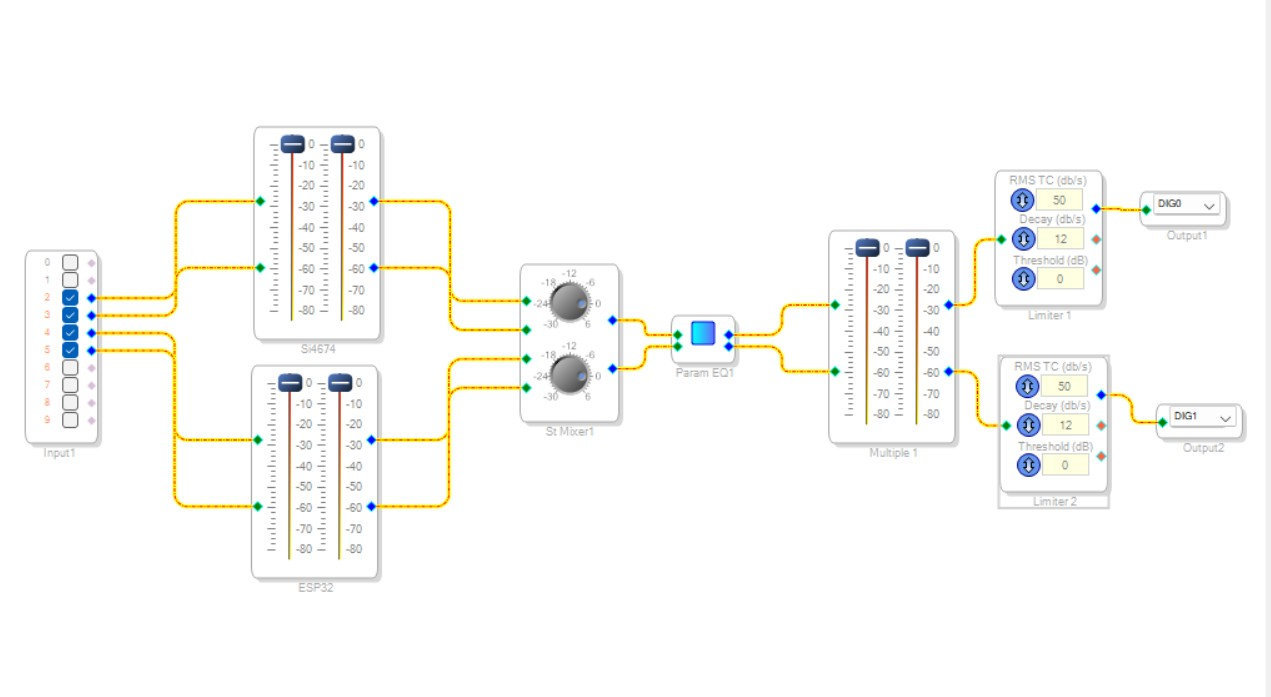
\includegraphics[width=\linewidth]{sigma-chain.jpg}
  \caption{The complete stereo signal-processing chain in SigmaStudio:
    Input \(\rightarrow\) source faders \(\rightarrow\) stereo mixer
    \(\rightarrow\) parametric EQ \(\rightarrow\) master volume
    \(\rightarrow\) per-channel limiters \(\rightarrow\) outputs.}
  \label{fig:ss-chain}
\end{figure}

\subsection{Block-by-block}

\begin{table}[htbp]
  \centering
  \small
  \begin{tabular}{@{}L{2.4cm}L{3.6cm}L{7.2cm}@{}}
    \drhead Stage & Block & Role \\
    \midrule
    Input      & Input (ch. 2--5)          & radio L/R, ESP32 L/R \\
    Source trim & Si4674, ESP32 faders     & per-source stereo level \\
    Mix        & Stereo Mixer             & combine sources, keep L/R \\
    EQ         & Parametric EQ (2-ch)     & high-pass + 5 peaking bands \\
    Volume     & Multiple volume (2-ch)   & master volume \\
    Protect    & Limiter 1 / Limiter 2    & per-channel peak limiting \\
    Output     & Output (DIG0, DIG1)      & L/R to FSC-BT1035 \\
    \bottomrule
  \end{tabular}
  \caption{Signal-processing blocks and their roles. The chain is stereo
    end to end; L and R never collapse to mono.}
  \label{tab:ss-blocks}
\end{table}

\subsection{Signal flow}

\begin{drcode}[Signal flow (stereo)]
Input ch2/3 (radio L/R)  -> Si4674 fader  --.
                                            |-> Stereo Mixer -> Param EQ
Input ch4/5 (ESP32 L/R)  -> ESP32  fader  --'
   -> Master Volume -> Limiter L / Limiter R -> Output DIG0 / DIG1 -> BT1035
\end{drcode}

\section{Equaliser}
\label{sec:ss-eq}

The parametric EQ is a two-channel (stereo) block; a single set of bands
applies identically to L and R. It is configured with one high-pass and
five peaking bands, all starting flat (0\,dB) so the default response is
neutral and any tone shaping is an explicit choice made at runtime by the
firmware.

\begin{table}[htbp]
  \centering
  \footnotesize
  \begin{tabular}{@{}L{1.4cm}L{2.4cm}L{2.2cm}L{1.6cm}L{1.2cm}@{}}
    \drhead Band & Type & Frequency & Gain & Q \\
    \midrule
    1 & HP Butterworth & 20\,Hz   & ---   & 1.41 \\
    2 & Peaking                      & 100\,Hz  & 0\,dB & 1.0 \\
    3 & Peaking                      & 400\,Hz  & 0\,dB & 1.0 \\
    4 & Peaking                      & 1\,kHz   & 0\,dB & 1.0 \\
    5 & Peaking                      & 3\,kHz   & 0\,dB & 1.0 \\
    6 & Peaking                      & 8\,kHz   & 0\,dB & 1.0 \\
    \bottomrule
  \end{tabular}
  \caption{Parametric EQ bands. Band~1 removes DC and subsonic content;
    bands 2--6 are the tone controls the firmware adjusts.}
  \label{tab:ss-eq}
\end{table}

\begin{drnote}[Double precision for the high-pass]
The high-pass sits at 20\,Hz, very low relative to the 48\,kHz sample
rate, so it uses a double-precision second-order block to avoid
coefficient-quantisation noise in the bass. The peaking bands can use
single precision.
\end{drnote}

\section{Master volume and limiters}
\label{sec:ss-vol}

A two-channel volume block provides the master level (0\,dB default). Two
single-channel limiters --- one per channel --- protect the FSC-BT1035
input from clipping on peaks. Suggested limiter settings are in
Table~\ref{tab:ss-lim}.

\begin{table}[htbp]
  \centering
  \begin{tabular}{@{}L{4.2cm}L{9.2cm}@{}}
    \drhead Parameter & Value \\
    \midrule
    RMS TC        & 50\,dB/s \\
    Decay         & 12\,dB/s \\
    Threshold     & $-1$\,dB (protective) \\
    \bottomrule
  \end{tabular}
  \caption{Per-channel limiter settings. The limiter is left fixed (not
    runtime-adjustable).}
  \label{tab:ss-lim}
\end{table}

\section{Runtime-controllable parameters}
\label{sec:ss-runtime}

The firmware controls a subset of the DSP at runtime via safeload writes.
These are the parameter cells whose addresses must be recorded from the
SigmaStudio export (Section~\ref{sec:ss-export}).

\begin{table}[htbp]
  \centering
  \begin{tabular}{@{}L{2.4cm}L{3.6cm}L{7.2cm}@{}}
    \drhead Control & Block & Runtime-adjustable \\
    \midrule
    Source levels (2)   & Si4674 / ESP32 faders & yes \\
    EQ bands 2--6       & Parametric EQ         & yes (gain/freq/Q) \\
    Master volume       & Multiple volume       & yes \\
    High-pass (band 1)  & Parametric EQ         & fixed \\
    Limiters            & Limiter 1 / 2         & fixed \\
    \bottomrule
  \end{tabular}
  \caption{Parameters exposed to the firmware. Fixed blocks are set once
    in the program and never written at runtime.}
  \label{tab:ss-runtime}
\end{table}

\section{Virtual enhancements (stereo depth and bass boost)}
\label{sec:ss-enhancements}

The SigmaStudio export does not include dedicated stereo widener or bass
boost blocks. Firmware maps enhancement levels (0--100) onto the
existing Param EQ1 bands at runtime:

\begin{itemize}
  \item \textbf{Bass enhance} --- peaking boost at 100\,Hz (+9\,dB max)
        and 400\,Hz (+3\,dB max).
  \item \textbf{Stereo enhance} --- slight 1\,kHz cut, plus 3\,kHz and
        8\,kHz lift for a wider, more present image. This is a
        psychoacoustic curve, not mid/side processing.
\end{itemize}

Enhancement levels are stored in \texttt{AudioProfile::enhancements} and
applied by \texttt{core::applyEnhancementsToEq()} before safeload. Base EQ
band settings in NVS are preserved; overlays replace affected bands only
while the corresponding level is greater than zero.

\begin{drcaution}[Use safeload for live changes]
All runtime updates to the volume, source levels, and EQ bands must go
through the ADAU1701 safeload mechanism. Writing parameter cells directly
while audio is playing produces audible clicks.
\end{drcaution}

\section{Exporting the program}
\label{sec:ss-export}

With the schematic complete, the program is exported for the firmware:

\begin{enumerate}
  \item Enable \emph{Action \(\rightarrow\) Enable Short Parameter Name
        for Export} so the exported cell names are concise.
  \item \emph{Action \(\rightarrow\) Export System Files}, and choose an
        output folder.
\end{enumerate}

The export produces the program data (control registers, program RAM, and
parameter RAM) as byte sequences, plus the symbolic parameter addresses.
The firmware's ADAU1701 driver replays the program data over
I\textsuperscript{2}C at boot, and uses the parameter addresses for
safeload updates.

\begin{drnote}[Export System Files vs. Link Compile Download]
Without a physical ADAU1701/USBi attached, \emph{Export System Files} is what
you want: it compiles the schematic and writes the files directly, with no
chip connection required. \emph{Link Compile Download} instead needs a live
communication channel to a chip --- either the classic USBi/ICP dongle, or
DigiRadio's own TCP:8086 SigmaStudio bridge (Section~\ref{sec:adau1701-sigmastudio-tcp})
when connecting live to a running board.
\end{drnote}

\section{Next revision: DigiRadioFinale}
\label{sec:ss-digiradiofinale}

\begin{drcaution}[Not yet integrated into firmware]
This section documents a SigmaStudio export (\texttt{DigiRadioFinale}) captured
2026-08-25 that is not yet the program the firmware replays at boot. It expands
the parameter RAM from 74 to 224 words with several new dedicated blocks,
replacing two of the EQ-overlay workarounds in
Section~\ref{sec:ss-enhancements} with real ADI algorithm modules. Driver,
safeload API, and this manual's runtime tables will be updated once the
program is finalised.
\end{drcaution}

\begin{figure}[htbp]
  \centering
  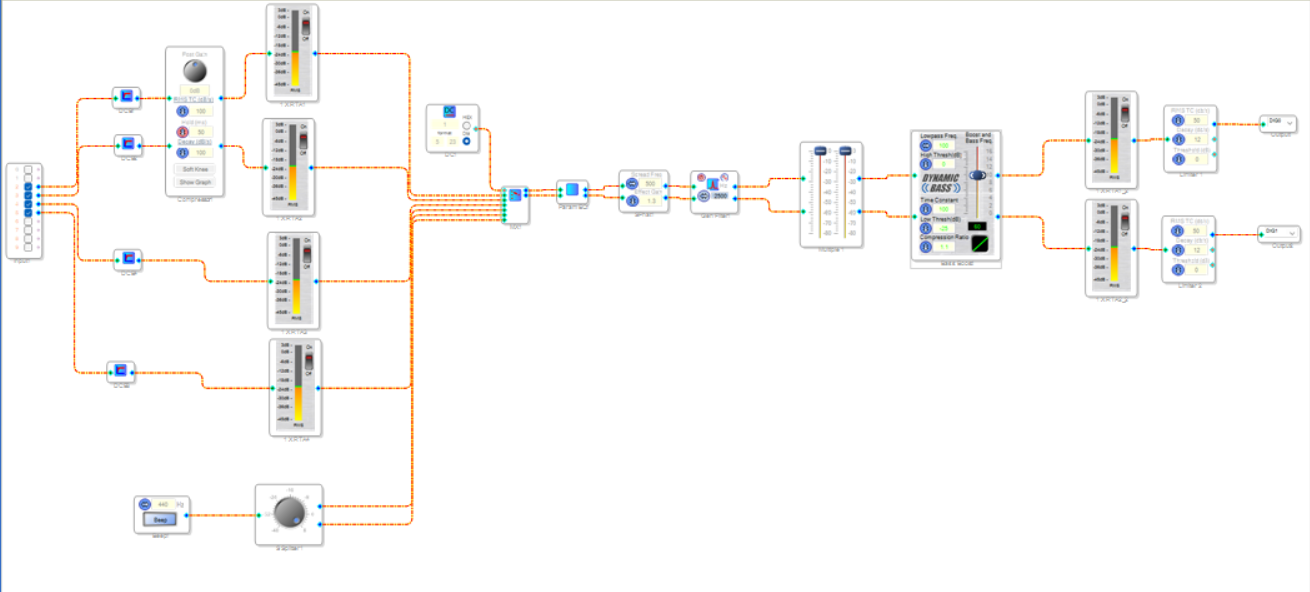
\includegraphics[width=\linewidth]{sigmastudiofinale.png}
  \caption{DigiRadioFinale signal chain: per-channel DC blockers and RMS
    compressor, four input-side level meters, the 6-leg Param EQ, the
    SuperPhat spatializer, an unconfigured general filter, master volume,
    the Dynamic Bass Boost algorithm, two output-side level meters, and the
    L/R limiters.}
  \label{fig:ss-digiradiofinale}
\end{figure}

\begin{table}[htbp]
  \centering
  \small
  \begin{tabular}{@{}L{2.6cm}L{2.2cm}L{7.6cm}@{}}
    \drhead Addresses & Block & Role \\
    \midrule
    0--2    & Beep1        & test tone (unchanged) \\
    3       & DC1          & input trim \\
    4--7    & DCB1--4      & DC blocker, one per channel \\
    8       & S Splitter1  & control fan-out (unchanged) \\
    9--46   & Compressor1  & RMS compander, 34-point curve \\
    47--58  & 1×RTA3,4,1,2 & 4 input-side level meters (readback) \\
    59--88  & Param EQ1    & 6 stereo legs (ST0--ST5) $\times$ 5 coefficients \\
    89--140 & SPhat1       & SuperPhat spatializer (dedicated algorithm,
                              replaces the stereo-enhance EQ overlay) \\
    141--145& Gen Filter1  & general 2nd-order filter, currently flat/bypassed
                              --- reserved, not yet configured (candidate slot
                              for Voice Clarifier) \\
    146--147& Multiple1    & master volume L/R (unchanged) \\
    148--187& Bass Boost1  & Dynamic Bass Boost algorithm (dedicated,
                              replaces the bass-enhance EQ overlay) \\
    188--193& 1×RTA2\_2,1\_2 & 2 output-side level meters (readback) \\
    194--223& Limiter2, Limiter1 & unchanged \\
    \bottomrule
  \end{tabular}
  \caption{DigiRadioFinale parameter RAM map, by address.}
  \label{tab:ss-digiradiofinale-map}
\end{table}

No dedicated mute cell exists yet in this export, and Gen Filter1 (the
Voice Clarifier candidate) is still an identity filter (b0=1, all other
coefficients zero). Both are pending further SigmaStudio work before this
program replaces the one described earlier in this chapter.

% ============================================================
%  DigiRadio — Manual section: Firmware Architecture
%  Drop this into the manual as a \section (or \chapter).
%
%  Required packages (add to the preamble if not present):
%    \usepackage{tikz}
%    \usetikzlibrary{positioning, arrows.meta, fit, backgrounds}
%    \usepackage{booktabs}   % for the interface table
%
%  The environments used here are standard. Replace itemize / framed
%  blocks with your own box taxonomy where you prefer.
% ============================================================

\chapter{Firmware Architecture}
\label{ch:firmware}
\label{sec:firmware-architecture}

The DigiRadio firmware runs on the ESP32-S3 and orchestrates three
companion chips into a single high-fidelity audio path: the Si4684
DAB+/FM tuner, the ADAU1701 SigmaDSP, and the FSC-BT1035 Bluetooth
transmitter. This section describes how the firmware is organised, how
audio flows through the system, and how each chip is controlled. The
day-to-day coding conventions (style, documentation, review rules) are
intentionally kept out of this manual and live in the repository's
\texttt{CONTRIBUTING.md} and \texttt{AGENTS.md}.

\section{Design principles}
\label{sec:fw-principles}

Two ideas shape the whole codebase:

\begin{itemize}
  \item \textbf{Strong typing.} Domain quantities (frequency, gain,
    station identifier, band) are dedicated types rather than raw
    integers or floats. Invalid states are made unrepresentable: input
    from the network, UART, or flash is validated once at the boundary
    into a domain type, and trusted thereafter.
  \item \textbf{Functional core, imperative shell.} All hardware-free
    logic --- coefficient math, boot-image framing, configuration
    parsing, station-list operations --- lives in a pure \emph{core}
    that compiles and is unit-tested on the host, with no dependency on
    ESP-IDF. Every access to the hardware (I\textsuperscript{2}C, SPI,
    UART, flash) lives in a thin \emph{shell} around that core. This
    keeps the logic testable without a board attached.
\end{itemize}

\section{Layered structure}
\label{sec:fw-layers}

The firmware is organised in three layers, with dependencies pointing
inward only (Figure~\ref{fig:fw-layers}). The outer shell may depend on
the services and the core; the pure core depends on nothing outside
itself.

\begin{figure}[htbp]
  \centering
  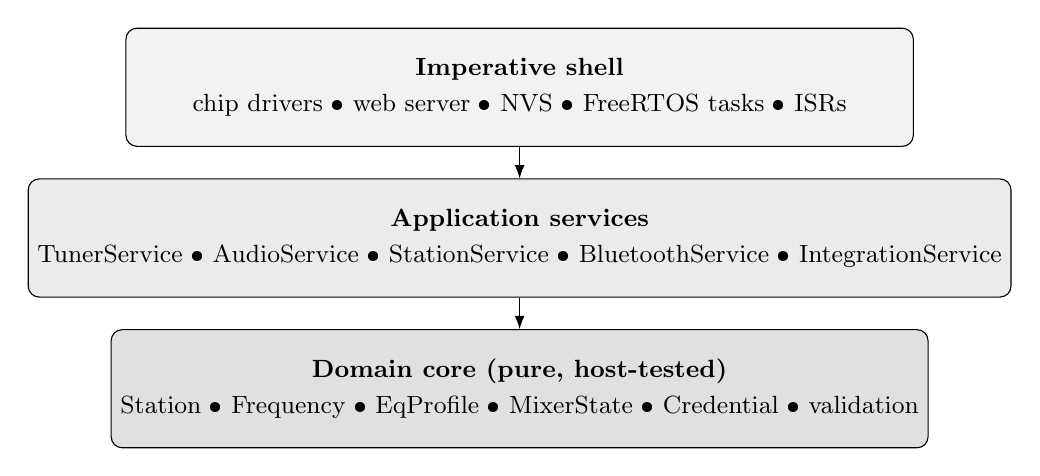
\begin{tikzpicture}[
      layer/.style={draw, rounded corners, minimum width=10cm,
        minimum height=1.5cm, align=center, font=\small},
      node distance=4mm]
    \node[layer, fill=black!5] (shell) {%
      \textbf{Imperative shell}\\[2pt]
      chip drivers \textbullet\ web server \textbullet\ NVS \textbullet\
      FreeRTOS tasks \textbullet\ ISRs};
    \node[layer, fill=black!8, below=of shell] (services) {%
      \textbf{Application services}\\[2pt]
      TunerService \textbullet\ AudioService \textbullet\
      StationService \textbullet\ BluetoothService \textbullet\
      IntegrationService};
    \node[layer, fill=black!12, below=of services] (core) {%
      \textbf{Domain core (pure, host-tested)}\\[2pt]
      Station \textbullet\ Frequency \textbullet\ EqProfile \textbullet\
      MixerState \textbullet\ Credential \textbullet\ validation};
    \draw[-{Latex}] (shell) -- (services);
    \draw[-{Latex}] (services) -- (core);
  \end{tikzpicture}
  \caption{Firmware layering. Dependencies point inward; the pure core
    has no hardware dependencies.}
  \label{fig:fw-layers}
\end{figure}

Application services take driver \emph{interfaces}
(\texttt{ITuner}, \texttt{IDsp}, \texttt{IBtModule},
\texttt{ISecureStore}) injected at construction. Because the services
depend on abstractions rather than concrete hardware, the same logic can
be exercised against fakes in host tests and against real silicon on the
device.

\section{Audio signal path}
\label{sec:fw-audio}

The audio chain is built around sound quality. The Si4684 produces the
DAB+/FM audio stream; the ADAU1701 applies equalisation and mixes it
with the ESP32 audio source; the FSC-BT1035 streams the result over
Bluetooth with aptX Adaptive (Figure~\ref{fig:fw-audio}).

\begin{figure}[htbp]
  \centering
  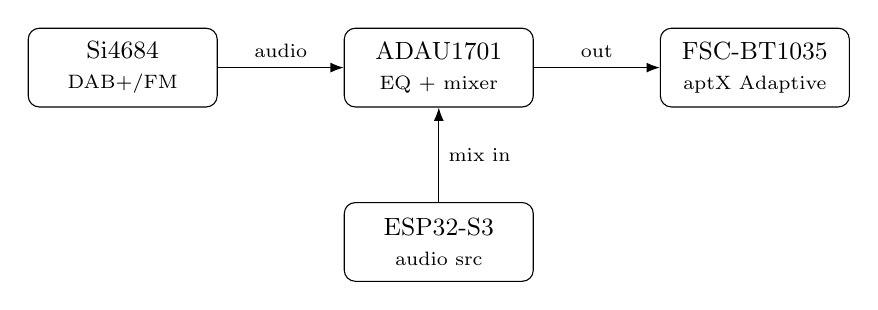
\begin{tikzpicture}[
      block/.style={draw, rounded corners, minimum height=1cm,
        minimum width=2.4cm, align=center, font=\small},
      >={Latex}, node distance=8mm]
    \node[block] (si) {Si4684\\\scriptsize DAB+/FM};
    \node[block, right=16mm of si] (dsp) {ADAU1701\\\scriptsize EQ + mixer};
    \node[block, right=16mm of dsp] (bt) {FSC-BT1035\\\scriptsize aptX Adaptive};
    \node[block, below=12mm of dsp] (esp) {ESP32-S3\\\scriptsize audio src};
    \draw[->] (si) -- (dsp) node[midway, above, font=\scriptsize]{audio};
    \draw[->] (dsp) -- (bt) node[midway, above, font=\scriptsize]{out};
    \draw[->] (esp) -- (dsp) node[midway, right, font=\scriptsize]{mix in};
  \end{tikzpicture}
  \caption{Audio signal path. The ADAU1701 input mixer selects/blends
    the Si4684 and ESP32 sources; equalisation is applied before the
    Bluetooth output stage.}
  \label{fig:fw-audio}
\end{figure}

Equalisation and input mixing are exposed to the rest of the firmware as
typed operations --- setting an EQ band from a gain, centre frequency,
and Q, or setting the mix level of a given source --- never as raw DSP
cell addresses. The biquad coefficient math runs in the pure core and is
verified against reference values in host tests.

\section{Chip control and boot}
\label{sec:fw-chips}

\paragraph{Si4684 (tuner).}
At power-up the driver follows the documented boot sequence: power on,
load the patch/bootloader, load the firmware image (FM or DAB), then
boot. Firmware images are large and are streamed to the chip in bounded
chunks from flash rather than buffered whole in RAM. See
Chapter~\ref{ch:si4684} for blob sources, uGreen extraction, and the full
\texttt{Si4684Driver} API (tuning, RSQ, DAB service list).

\paragraph{ADAU1701 (DSP).}
The board carries no self-boot EEPROM. Instead, the ESP32 writes the
SigmaStudio-exported program into the DSP's RAM at \emph{every} boot.
Runtime changes to equalisation and mixing use the ADAU1701 safeload
mechanism, so parameter updates are click-free while audio is playing.
Which blocks are runtime-controllable (source faders, EQ bands 2--6,
master volume) versus fixed at export (high-pass, limiters) is listed in
Chapter~\ref{ch:sigmastudio}, Section~\ref{sec:ss-runtime}. The full driver
stack, parameter map, \texttt{AudioService}, and HTTP routes are documented
in Chapter~\ref{ch:adau1701}.

\begin{drcaution}[Safeload]
Writing DSP parameter cells directly while audio is running produces
audible clicks. All runtime EQ and mixer changes must go through the
safeload registers.
\end{drcaution}

\paragraph{FSC-BT1035 (Bluetooth).}
The module is controlled by AT commands over UART with hardware flow control.
The initialisation sequence includes enabling I\textsuperscript{2}S slave mode
(\texttt{AT+AUXCFG=3} and \texttt{AT+I2SCFG=67}), which is required for the
wired digital audio path from the ADAU1701 to the module.
Command responses are parsed explicitly, with timeouts treated as errors.
Full driver API, boot flow, and error codes are in Chapter~\ref{ch:bt1035}.

\section{Configuration, storage, and user interface}
\label{sec:fw-config}

Network provisioning is implemented as an explicit state machine
(\texttt{net::NetState}): on first boot (or when STA join fails) the
device opens a setup SoftAP (\texttt{DigiRadio-setup}) and serves a
minimal gzipped web UI from flash. After the user submits credentials via
\texttt{POST /api/wifi}, values are validated in the pure core, persisted
through \texttt{core::ISecureStore}, and the device reboots into STA mode
on the next boot. The HTTP endpoints and JSON schemas are documented in
Chapter~\ref{ch:api}.

\paragraph{Implemented (fw 0.8.3).}
\begin{itemize}
  \item \textbf{Network} --- \texttt{GET /api/health}, \texttt{POST /api/wifi},
        SoftAP/STA state machine (\texttt{NetState}), tabbed gzipped web UI.
  \item \textbf{Tuner} --- \texttt{/api/tuner/*} (FM/DAB tune, seek, services,
        play); RDS and DAB dynamic labels in status JSON.
  \item \textbf{Audio} --- \texttt{/api/audio/*} (profile, reset, stereo/bass
        enhance); six-band EQ via \texttt{AudioService}.
  \item \textbf{Bluetooth} --- \texttt{/api/bluetooth/*} (pair, stop, disconnect,
        status).
  \item \textbf{Presets} --- \texttt{/api/stations/*} including reorder and
        integrated recall via \texttt{IntegrationService}.
  \item \textbf{Storage} --- \texttt{NvsSecureStore}, \texttt{NvsAudioProfileStore},
        encrypted NVS + flash encryption (development mode); keys in
        \texttt{nvs\_keys} partition; init via \texttt{initEncryptedStorage()}.
\end{itemize}

\paragraph{Legacy note (Slices 1--2).}
The first slices introduced health, Wi-Fi provisioning, and the secure-store
boundary; the bullets above supersede the original slice-scoped list.

Sensitive data uses \texttt{core::Secret} where applicable so values cannot
be logged or implicitly converted to a string; buffers are cleared on
destruction. Firmware~0.8.3 enables NVS and flash encryption at rest via
\texttt{secure\_store::initEncryptedStorage()} (see
\texttt{docs/security-flash-nvs.md} and Chapter~\ref{sec:api-storage}).

\section{Companion-chip boot at power-up}
\label{sec:fw-chip-boot}

The ESP32-S3 loads both audio companion chips from assets under
\texttt{Software/Firmware/} during \texttt{app\_main}, before network
bring-up:

\begin{enumerate}
  \item \textbf{Si4684} (SPI): ROM patch \texttt{rom\_patch\_016.bin}, then either
    DAB image \texttt{dab\_firmware.bin} or FM image \texttt{fm\_firmware.bin},
    following AN649 (Chapter~\ref{ch:si4684}). DAB blob default from PE5PVB; FM
    from eval pack or uGreen \texttt{radio\_cli}. Blobs are local-only
    (\texttt{.gitignore}); embedded via ESP-IDF \texttt{EMBED\_FILES}.
  \item \textbf{ADAU1701} (I\textsuperscript{2}C): SigmaStudio export
    (\texttt{DigiRadio\_IC\_1.h}) replayed through
    \texttt{SIGMA\_WRITE\_REGISTER\_BLOCK} after hardware reset. The DSP
    program lives in RAM only; download runs on every boot
    (Chapter~\ref{ch:adau1701}, Section~\ref{sec:adau1701-boot}).
  \item \textbf{Audio profile}: \texttt{audio::AudioService::loadAndApply()}
    restores the saved \texttt{core::AudioProfile} from NVS (or factory
    defaults) via ADAU1701 safeload before network bring-up.
  \item \textbf{FSC-BT1035} (UART): \texttt{bt1035::Bt1035Driver::boot()}
    enables I\textsuperscript{2}S slave mode (\texttt{AT+AUXCFG=3},
    \texttt{AT+I2SCFG=67}) after the DSP path is configured
    (Chapter~\ref{ch:bt1035}).
\end{enumerate}

If either driver returns an error, the firmware logs the failure and stops
before starting Wi-Fi (fail-closed bring-up).

\section{Error-handling model}
\label{sec:fw-errors}

Every operation that can fail returns a typed result
(\texttt{std::expected<T, Error>}); nothing fails silently and every
timeout is an explicit error value. Errors propagate to the layer that
can act on them --- a driver reports, a service decides (retry, degrade,
or surface to the UI), and the top level logs. C++ exceptions are
disabled.

\section{Toolchain}
\label{sec:fw-toolchain}

\begin{table}[htbp]
  \centering
  \begin{tabular}{@{}ll@{}}
    \toprule
    \textbf{Item} & \textbf{Choice} \\
    \midrule
    Framework        & ESP-IDF v5.5.x (native) \\
    Language          & C++23 (\texttt{-std=gnu++23}) \\
    Error model       & \texttt{std::expected}; exceptions off \\
    Hardware licence  & CERN-OHL-S v2 \\
    Firmware licence  & Apache-2.0 \\
    \bottomrule
  \end{tabular}
  \caption{Firmware toolchain and licensing summary.}
  \label{tab:fw-toolchain}
\end{table}

The firmware source, build instructions, and development conventions are
maintained in the \texttt{Software/} directory of the project
repository.

% ============================================================
%  DigiRadio — Manual chapter: Si4684 tuner
% ============================================================

\chapter{Si4684 DAB+/FM Tuner}
\label{ch:si4684}

The Skyworks Si4684 is the primary RF front-end of DigiRadio: it demodulates
DAB/DAB+ and FM, decodes RDS, and delivers PCM over I\textsuperscript{2}S to
the ADAU1701. This chapter documents how firmware images are obtained and kept
local, how the chip is booted on the ESP32-S3, and how \texttt{Si4684Driver}
exposes every day-to-day operation without leaking register-level details to
application code.

\section{Role in the audio chain}
\label{sec:si4684-role}

After boot the Si4684 runs as an I\textsuperscript{2}S master at
44.1\,kHz stereo. The ESP32 loads proprietary application firmware into chip
RAM at every cold start (there is no self-boot EEPROM on DigiRadio). Tuning,
service selection, and signal-quality reads all go through
\texttt{si4684::Si4684Driver}; higher layers (\texttt{TunerService}, web UI)
will depend on that class rather than issuing SPI transactions directly.

\begin{drref}[Programming guide]
Command opcodes, property IDs, and reply layouts follow Skyworks application
note \textbf{AN649} (Si468x programming guide). The DigiRadio driver aligns
with the PE5PVB/SI4684-DAB-Receiver reference for DAB and with community FM
images for the FM application blob.
\end{drref}

\section{Firmware images}
\label{sec:si4684-firmware}

Three binary blobs live under \texttt{Firmware/Si4684-Firmware/}. They are
\textbf{not} committed to the public Git repository (proprietary Skyworks /
uGreen licence); \texttt{.gitignore} keeps them on the developer machine only.

\begin{table}[htbp]
  \centering
  \begin{tabular}{@{}llp{6.2cm}@{}}
    \toprule
    \textbf{Local file} & \textbf{Typ.\ size} & \textbf{Source} \\
    \midrule
    \texttt{rom\_patch\_016.bin} & 5796 B &
      ROM patch (\texttt{rom00\_patch.016.bin}); refreshed from
      PE5PVB or uGreen \texttt{radio\_cli}. \\
    \texttt{dab\_firmware.bin} & $\sim$517--497 KB &
      DAB application image; default from PE5PVB header extract; optional
      uGreen \texttt{dab\_radio\_6\_0\_6.bin}. \\
    \texttt{fm\_firmware.bin} & $\sim$530 KB &
      FM/HD application; eval CD, dabpi \texttt{si46xx\_firmware/}, or uGreen
      \texttt{fmhd\_radio\_5\_1\_3.bin}. \\
    \bottomrule
  \end{tabular}
  \caption{Si4684 firmware blobs (local only).}
  \label{tab:si4684-blobs}
\end{table}

\subsection{Where images come from}
\label{sec:si4684-sources}

Community projects name the same Skyworks files differently; none of them
redistribute the binaries in git:

\begin{itemize}
  \item \textbf{PE5PVB/SI4684-DAB-Receiver} --- DAB image and ROM patch as
    C arrays (\texttt{firmware.h}, \texttt{Si468xROM.h}). Safe to automate.
  \item \textbf{uGreen DABBoard} (\url{https://ugreen.eu/downloads/}) ---
    \texttt{Files\_v16.zip} embeds FM, DAB, and patch inside
    \texttt{radio\_cli}; use \texttt{tools/extract\_ugreen\_radio\_cli.py}.
  \item \textbf{hitech95/si468x\_dab\_receiver} --- Linux driver only; device
    tree references \texttt{si468x/fmhd\_radio\_5\_1\_0.bin} but does not
    ship the files (closed source).
  \item \textbf{PhilBladen/Radio} --- STM32 reference using \emph{external}
    SPI flash (\texttt{FLASH\_LOAD}); different hardware path from DigiRadio's
    \texttt{HOST\_LOAD} flow.
\end{itemize}

\begin{drcaution}[Licence]
Do not push \texttt{*.bin} firmware to GitHub. Obtain images from your own
eval board, uGreen customer download, or dabpi folder; keep them in
\texttt{Firmware/Si4684-Firmware/} locally.
\end{drcaution}

\subsection{Refreshing blobs}
\label{sec:si4684-refresh}

\begin{verbatim}
# DAB + patch from PE5PVB (always safe to re-run):
python3 tools/fetch_si4684_firmware.py --dab-only

# FM from uGreen radio_cli (Files_v16.zip):
python3 tools/fetch_si4684_firmware.py \
    --from-ugreen-radio-cli ~/Downloads/Files_v16.zip

# All three blobs from uGreen (overrides PE5PVB DAB):
python3 tools/fetch_si4684_firmware.py \
    --from-ugreen-radio-cli ~/Downloads/Files_v16.zip --ugreen-all

# FM from dabpi / Skyworks eval folder:
python3 tools/fetch_si4684_firmware.py --si46xx-dir /path/to/si46xx_firmware
\end{verbatim}

Low-level helpers: \texttt{tools/extract\_si4684\_blob.py} (C header or copy),
\texttt{tools/extract\_ugreen\_radio\_cli.py} (ELF symbol scrape).

\section{Boot sequence (HOST\_LOAD)}
\label{sec:si4684-boot}

DigiRadio follows AN649 ``cold start with HOST\_LOAD'' (same as PE5PVB), not
the \texttt{FLASH\_LOAD} path used by boards with a pre-programmed SST25V.

\begin{figure}[htbp]
  \centering
  \begin{tikzpicture}[
      step/.style={draw, rounded corners, minimum width=9cm,
        minimum height=0.9cm, align=center, font=\small},
      >={Latex}, node distance=3mm]
    \node[step, fill=black!6] (rst) {Hardware reset (RST\#)};
    \node[step, fill=black!6, below=of rst] (pu)
      {POWER\_UP (crystal / clock args)};
    \node[step, fill=black!6, below=of pu] (li1) {LOAD\_INIT};
    \node[step, fill=black!8, below=of li1] (patch)
      {HOST\_LOAD \texttt{rom\_patch\_016.bin} (124 B chunks)};
    \node[step, fill=black!6, below=of patch] (li2) {LOAD\_INIT};
    \node[step, fill=black!8, below=of li2] (img)
      {HOST\_LOAD \texttt{dab\_} or \texttt{fm\_firmware.bin}
       (2044 B chunks)};
    \node[step, fill=black!6, below=of img] (boot) {BOOT};
    \node[step, fill=black!10, below=of boot] (cfg)
      {Properties: I\textsuperscript{2}S 44.1 kHz, RDS/DAB FE, volume};
    \foreach \a/\b in {rst/pu, pu/li1, li1/patch, patch/li2, li2/img,
      img/boot, boot/cfg} {
      \draw[->] (\a) -- (\b);
    }
  \end{tikzpicture}
  \caption{Si4684 boot flow on DigiRadio (AN649 / PE5PVB).}
  \label{fig:si4684-boot}
\end{figure}

Images are embedded in the ESP32 flash partition via ESP-IDF
\texttt{EMBED\_FILES} and streamed through \texttt{IFirmwareBlobReader} so the
full $\sim$1\,MB of patch + DAB + FM never has to fit in RAM at once. Switching
band (\texttt{Si4684Band::Fm} $\leftrightarrow$ \texttt{Dab}) performs reset and
a complete reload of patch + the other application image.

\section{Si4684Driver API}
\label{sec:si4684-driver}

\texttt{Si4684Driver} owns SPI, implements boot, and exposes intent-level
methods grouped below. All return \texttt{std::expected<T, Si4684Error>}; FM
calls fail with \texttt{WrongBand} if the FM image is not loaded, and vice
versa for DAB.

\subsection{Bring-up and diagnostics}

\begin{table}[htbp]
  \centering
  \begin{tabular}{@{}ll@{}}
    \toprule
    \textbf{Method} & \textbf{Purpose} \\
    \midrule
    \texttt{boot(Si4684Band)} & Cold start + default properties \\
    \texttt{isBooted()}, \texttt{loadedBand()} & State query \\
    \texttt{getPartInfo()} & Chip ID + firmware version \\
    \texttt{getSysState()} & Running application type \\
    \texttt{setProperty(id, value)} & Generic SET\_PROPERTY \\
    \texttt{setVolume(0--63)} & Audio attenuator \\
    \bottomrule
  \end{tabular}
  \caption{Si4684 bring-up and property access.}
\end{table}

\subsection{FM operations}

Requires \texttt{boot(Si4684Band::Fm)}.

\begin{itemize}
  \item \texttt{tuneFm(frequencyKhz)} --- FM\_TUNE\_FREQ, waits for STC.
  \item \texttt{seekFm(up, wrap)} --- FM\_SEEK\_START; returns tuned kHz.
  \item \texttt{readFmRsq()} --- RSSI, SNR, stereo flag, validity.
  \item \texttt{readFmRds()} --- last RDS group blocks A--D (FIFO depth).
  \item \texttt{readDabServiceData(statusOnly, ack)} --- DAB data-service
    payload (DLS when \texttt{DATA\_SRC=2}).
\end{itemize}

\subsection{DAB operations}

Requires \texttt{boot(Si4684Band::Dab)}. The default Band~III frequency plan
(38 channels, Table~\ref{tab:si4684-dab-plan}) is installed automatically
after boot.

\begin{itemize}
  \item \texttt{installDefaultDabFrequencyPlan()} --- DAB\_SET\_FREQ\_LIST
    (also called from boot).
  \item \texttt{tuneDab(freqIndex)} --- tune ensemble by index 0--37.
  \item \texttt{readDabDigRadStatus()} --- FIC quality, CNR, lock.
  \item \texttt{readDabEventStatus()} --- service-list-ready flag.
  \item \texttt{fetchDabServiceList()} --- parsed services + labels.
  \item \texttt{startDabService(serviceId, componentId)} --- begin audio
    decode (START\_DIGITAL\_SERVICE).
\end{itemize}

\begin{table}[htbp]
  \centering
  \small
  \begin{tabular}{@{}cl@{}}
    \toprule
    \textbf{Index} & \textbf{Centre frequency (kHz)} \\
    \midrule
    0--3   & 174928 -- 180064 (5A--5D) \\
    4--7   & 181936 -- 187072 (6A--6D) \\
    8--11  & 188928 -- 194064 (7A--7D) \\
    12--15 & 195936 -- 201072 (8A--8D) \\
    16--19 & 202928 -- 208064 (9A--9D) \\
    20--23 & 209936 -- 215072 (10A--10D) \\
    24--27 & 216928 -- 222064 (11A--11D) \\
    28--31 & 223936 -- 229072 (12A--12D) \\
    32--35 & 230784 -- 235776 (13A--13D) \\
    36--37 & 237488 -- 239200 (13E--13F) \\
    \bottomrule
  \end{tabular}
  \caption{DAB Band III plan (\texttt{kDefaultDabFrequencyKhz}).}
  \label{tab:si4684-dab-plan}
\end{table}

\subsection{Typical DAB session}
\label{sec:si4684-dab-session}

\begin{enumerate}
  \item \texttt{boot(Dab)} at power-up (already done in
    \texttt{HardwareBootstrap}).
  \item \texttt{tuneDab(index)} for the desired ensemble (Band III index
    0--37, Table~\ref{tab:si4684-dab-plan}).
  \item Poll \texttt{readDabDigRadStatus()} until FIC quality $> 0$.
  \item \texttt{fetchDabServiceList()} when
    \texttt{readDabEventStatus().serviceListReady}.
  \item \texttt{startDabService(serviceId, componentId)} for the chosen
    programme; PCM appears on I\textsuperscript{2}S to the ADAU1701.
\end{enumerate}

\begin{drnote}[DAB, not DVB]
DigiRadio receives \textbf{DAB/DAB+} (Digital \emph{Audio} Broadcasting),
not DVB-T/T2 video. Tuning is by ensemble frequency index and digital
service/component IDs --- there is no transport-stream PAT/PMT scan like
DVB-T.
\end{drnote}

\subsection{Typical FM session}
\label{sec:si4684-fm-session}

FM requires the FM application image loaded at boot
(\texttt{boot(Si4684Band::Fm)}). DigiRadio defaults to DAB at power-up;
switching to FM reloads patch + \texttt{fm\_firmware.bin} (full HOST\_LOAD).

\begin{enumerate}
  \item \texttt{boot(Fm)} --- resets the chip and loads the FM image.
  \item \texttt{tuneFm(frequencyKhz)} --- e.g.\ 101500 for 101.5\,MHz;
        waits for seek/tune complete (STC).
  \item \texttt{readFmRsq()} --- RSSI, SNR, stereo flag, validity.
  \item Optional: \texttt{seekFm(up, wrap)} --- scan to next station.
  \item Optional: \texttt{readFmRds()} --- last RDS group (PI, PS, RT).
\end{enumerate}

FM audio is emitted on the same I\textsuperscript{2}S pins as DAB once the
FM image is running.

\subsection{Choosing DAB or FM}
\label{sec:si4684-band-choice}

Only one application image runs at a time. \texttt{Si4684Driver::boot(band)}
selects the blob:

\begin{table}[htbp]
  \centering
  \begin{tabular}{@{}lll@{}}
    \drhead Band & Image loaded & Primary API \\
    \midrule
    \texttt{Si4684Band::Dab} & \texttt{dab\_firmware.bin} &
      \texttt{tuneDab}, service list, \texttt{startDabService} \\
    \texttt{Si4684Band::Fm}  & \texttt{fm\_firmware.bin} &
      \texttt{tuneFm}, \texttt{seekFm}, RSQ, RDS \\
    \bottomrule
  \end{tabular}
  \caption{Band-specific firmware and driver entry points.}
  \label{tab:si4684-band-api}
\end{table}

Calling an FM method while the DAB image is loaded (or vice versa) returns
\texttt{Si4684Error::WrongBand}. Switching band performs reset and a complete
HOST\_LOAD of patch + the other image ($\sim$1\,s).

\subsection{HTTP API mapping (web UI)}
\label{sec:si4684-http}

The setup UI and REST clients use \texttt{tuner::TunerService}, which wraps
\texttt{Si4684Tuner} (Chapter~\ref{ch:api}). Summary:

\begin{table}[htbp]
  \centering
  \small
  \begin{tabular}{@{}llp{5.5cm}@{}}
    \drhead Endpoint & Band & Action \\
    \midrule
    \texttt{POST /api/tuner/tune} &
      DAB & \texttt{\{"band":"dab","freq\_index":0..37\}} \\
    \texttt{POST /api/tuner/tune} &
      FM  & \texttt{\{"band":"fm","frequency\_khz":64000..108000\}} \\
    \texttt{GET /api/tuner/services} & DAB only & Programme list for ensemble \\
    \texttt{POST /api/tuner/play}    & DAB only & Start \texttt{service\_id}/\texttt{component\_id} \\
    \texttt{POST /api/tuner/seek}    & FM only  & Seek up, return new kHz \\
    \texttt{GET /api/tuner/status}   & both     & Locked state, RSQ or DIGRAD \\
    \bottomrule
  \end{tabular}
  \caption{Tuner HTTP routes vs band (full schemas in Chapter~\ref{ch:api}).}
  \label{tab:si4684-http}
\end{table}

\begin{drnote}[FM tune via HTTP today]
\texttt{POST /api/tuner/tune} with \texttt{band:"fm"} calls
\texttt{TunerService::tuneFm}, which may trigger a band reload if the device
booted in DAB. Plan station presets and automatic band selection in a later
slice.
\end{drnote}

\section{Integration at power-up}
\label{sec:si4684-integration}

\texttt{main/hardware\_bootstrap.cpp} constructs a static
\texttt{Si4684EmbeddedImages}, \texttt{Si4684Driver}, and
\texttt{Si4684Tuner}, calls \texttt{boot(Si4684Band::Dab)} before Wi-Fi,
then boots the ADAU1701. Failure is fail-closed (logged, no network start).
\texttt{main/main.cpp} wraps the tuner adapter in
\texttt{tuner::TunerService} and passes it to \texttt{NetBootstrap::start()}
so HTTP routes under \texttt{/api/tuner/*} can tune and play at runtime.

\section{Further reading}
\label{sec:si4684-reading}

\begin{itemize}
  \item Skyworks AN649 --- command and property reference.
  \item \texttt{Firmware/Si4684-Firmware/README.md} --- blob refresh cheatsheet.
  \item PE5PVB \texttt{si4684.cpp} --- DAB service list and MOT (not yet ported).
  \item uGreen \texttt{radio\_cli\_RELEASE\_NOTES.md} --- embedded firmware versions.
\end{itemize}

% ============================================================
%  DigiRadio — Manual chapter: ADAU1701 DSP
% ============================================================

\chapter{ADAU1701 Audio DSP}
\label{ch:adau1701}

The Analog Devices ADAU1701 is the central audio processor of DigiRadio: it
mixes the Si4684 radio stream with the ESP32 I\textsuperscript{2}S source,
applies parametric equalisation and master volume, and feeds the
FSC-BT1035 over I\textsuperscript{2}S. This chapter documents how the
SigmaStudio program is stored and replayed at boot, how
\texttt{adau1701::Adau1701Driver} controls the chip over I\textsuperscript{2}C,
and how application code (\texttt{audio::AudioService}, HTTP, web UI) uses the
driver without touching parameter RAM addresses directly.

\begin{drref}[Companion chapter]
The SigmaStudio \emph{design} --- hardware settings, signal chain, EQ bands,
and export procedure --- is documented in Chapter~\ref{ch:sigmastudio}. This
chapter covers the \emph{firmware side}: boot, safeload, driver API, domain
types, persistence, and HTTP integration.
\end{drref}

\section{Role in the audio chain}
\label{sec:adau1701-role}

After boot the ADAU1701 runs as the I\textsuperscript{2}S \textbf{master}
at 48\,kHz, 24-bit stereo. It receives PCM from the Si4684 on serial input~0
and from the ESP32 on serial input~1, mixes and equalises the result, and
outputs to the Bluetooth module on \texttt{SDATA\_OUT0}. The ESP32 never
processes audio samples in software; all tone shaping and mixing happen inside
the DSP program exported from SigmaStudio.

Every runtime adjustment --- input level, EQ band, master volume, stereo/bass
enhancement --- flows through typed domain objects in \texttt{components/core}
and reaches the hardware only via \texttt{Adau1701Driver} safeload writes.
Board wiring and I\textsuperscript{2}C address are in
Section~\ref{sec:hw-adau} (Chapter~\ref{ch:hardware}).

\section{Program image (SigmaStudio export)}
\label{sec:adau1701-firmware}

Unlike the Si4684 blobs (local-only, not in git), the ADAU1701 export is
\textbf{committed} under \texttt{Firmware/ADAU1701-Firmware/}. It is the
authoritative DSP program for firmware builds.

\begin{table}[htbp]
  \centering
  \begin{tabular}{@{}llp{6.5cm}@{}}
    \toprule
    \textbf{File} & \textbf{Role} & \textbf{Used by firmware} \\
    \midrule
    \texttt{DigiRadio\_IC\_1.h} &
      Program + parameter RAM init data &
      \texttt{default\_download\_IC\_1()} replayed at boot \\
    \texttt{DigiRadio\_IC\_1\_PARAM.h} &
      Parameter cell indices &
      \texttt{ADDR\_*} macros; safeload targets \\
    \texttt{DigiRadio\_IC\_1\_REG.h} &
      Control register map &
      Safeload trigger registers \\
    \texttt{DigiRadio\_NetList.xml} &
      Schematic netlist &
      Reference when re-exporting \\
    \texttt{DigiRadio.params} &
      Parameter metadata &
      SigmaStudio round-trip \\
    \texttt{SigmaStudioFW.h} &
      Safeload / I2C glue header &
      \texttt{sigma\_safeload\_*} API \\
    \bottomrule
  \end{tabular}
  \caption{ADAU1701 SigmaStudio export files (in git).}
  \label{tab:adau1701-files}
\end{table}

The driver component wraps the generated C in three layers:
\texttt{adau1701\_program.c} calls \texttt{default\_download\_IC\_1()};
\texttt{SigmaStudioFW.c} implements \texttt{SIGMA\_WRITE\_REGISTER\_BLOCK}
and safeload on ESP-IDF I\textsuperscript{2}C; \texttt{Adau1701Driver.cpp}
adds reset, boot state, and typed runtime control.

\subsection{Refreshing after a SigmaStudio change}
\label{sec:adau1701-refresh}

When the schematic changes in SigmaStudio (new block, different EQ layout,
renamed cells):

\begin{enumerate}
  \item Edit the project offline (Chapter~\ref{ch:sigmastudio},
        Section~\ref{sec:ss-export}).
  \item \emph{Action $\rightarrow$ Export System Files} into
        \texttt{Firmware/ADAU1701-Firmware/}, overwriting the generated headers.
  \item Copy or reconcile any new \texttt{ADDR\_*} symbols into
        \texttt{Adau1701ParamMap.hpp} if block names moved (fader/EQ addresses
        must match \texttt{DigiRadio\_IC\_1\_PARAM.h}).
  \item Rebuild firmware; the ESP32 will replay the new download on next boot.
  \item Update Chapter~\ref{ch:sigmastudio} tables if band frequencies or the
        signal chain changed.
\end{enumerate}

\begin{drnote}[No USBi download on DigiRadio]
Do \emph{not} rely on SigmaStudio \emph{Link Compile Download} on this
hardware path. Export-only workflow is sufficient: the ESP32 is the programmer
at every power-up.
\end{drnote}

\section{Boot sequence (I\textsuperscript{2}C RAM load)}
\label{sec:adau1701-boot}

DigiRadio has no ADAU1701 self-boot EEPROM. The ESP32 holds the only copy of
the DSP program and writes it into RAM after each reset.

\begin{figure}[htbp]
  \centering
  \begin{tikzpicture}[
      step/.style={draw, rounded corners, minimum width=9.5cm,
        minimum height=0.9cm, align=center, font=\small},
      >={Latex}, node distance=3mm]
    \node[step, fill=black!6] (rst) {Assert RESET\# (10\,ms), release};
    \node[step, fill=black!6, below=of rst] (i2c)
      {Create I\textsuperscript{2}C master @ 100\,kHz, address 0x34};
    \node[step, fill=black!8, below=of i2c] (dl)
      {\texttt{default\_download\_IC\_1()} --- control, program, param RAM};
    \node[step, fill=black!6, below=of dl] (ready)
      {\texttt{Adau1701Driver::isBooted()} = true};
    \node[step, fill=black!10, below=of ready] (prof)
      {\texttt{AudioService::loadAndApply()} --- safeload user profile};
    \foreach \a/\b in {rst/i2c, i2c/dl, dl/ready, ready/prof} {
      \draw[->] (\a) -- (\b);
    }
  \end{tikzpicture}
  \caption{ADAU1701 boot flow on DigiRadio (host RAM load).}
  \label{fig:adau1701-boot}
\end{figure}

\texttt{SIGMA\_WRITE\_REGISTER\_BLOCK} streams each write in 64-byte I\textsuperscript{2}C
chunks. After download, \texttt{loadAndApply()} restores the saved
\texttt{core::AudioProfile} from NVS (or factory defaults) so user settings
survive power cycles without re-writing the whole program.

\section{Software architecture}
\label{sec:adau1701-stack}

Application code never includes \texttt{DigiRadio\_IC\_1\_PARAM.h}. The stack
separates concerns as follows:

\begin{table}[htbp]
  \centering
  \small
  \begin{tabular}{@{}llp{5.8cm}@{}}
    \drhead Layer & Type & Responsibility \\
    \midrule
    HTTP / UI       & \texttt{SetupWebServer}, web UI &
      JSON $\rightarrow$ \texttt{AudioService} \\
    Service         & \texttt{audio::AudioService} &
      Profile in RAM, NVS, enhancement overlay \\
    Domain          & \texttt{core::AudioProfile}, \texttt{IDsp} &
      Host-testable types, no ESP-IDF \\
    Adapter         & \texttt{adau1701::Adau1701Dsp} &
      Maps \texttt{DspError} $\leftrightarrow$ \texttt{Adau1701Error} \\
    Driver          & \texttt{adau1701::Adau1701Driver} &
      I\textsuperscript{2}C, boot, safeload \\
    Generated + glue & \texttt{DigiRadio\_IC\_1.h}, \texttt{SigmaStudioFW.c} &
      SigmaStudio export, register writes \\
    \bottomrule
  \end{tabular}
  \caption{ADAU1701 control stack (Slice~5).}
  \label{tab:adau1701-stack}
\end{table}

\texttt{AudioService} merges \texttt{AudioProfile::enhancements} into the
effective EQ via \texttt{core::applyEnhancementsToEq()} before calling
\texttt{IDsp::applyEq()} or \texttt{applyProfile()}. Base EQ settings in NVS
stay unchanged; enhancement bands are overlays (Section~\ref{sec:ss-enhancements}).

\section{Adau1701Driver API}
\label{sec:adau1701-driver}

\texttt{Adau1701Driver} owns the I\textsuperscript{2}C bus (RAII), drives
RESET\#, and exposes intent-level methods. All return
\texttt{std::expected<T, Adau1701Error>}. Runtime methods require a prior
successful \texttt{boot()}.

\subsection{Bring-up and state}

\begin{table}[htbp]
  \centering
  \begin{tabular}{@{}ll@{}}
    \toprule
    \textbf{Method} & \textbf{Purpose} \\
    \midrule
    \texttt{boot()} & Reset chip, init I\textsuperscript{2}C, run
      \texttt{default\_download\_IC\_1()} \\
    \texttt{isBooted()} & \texttt{true} after successful download \\
    \bottomrule
  \end{tabular}
  \caption{ADAU1701 bring-up.}
\end{table}

\subsection{Full profile and partial updates}

\begin{table}[htbp]
  \centering
  \begin{tabular}{@{}ll@{}}
    \toprule
    \textbf{Method} & \textbf{Purpose} \\
    \midrule
    \texttt{applyProfile(profile)} &
      Safeload mixer + EQ + master in one call \\
    \texttt{applyMixer(mixer)} &
      Si4684/ESP32 faders + St Mixer1 L/R \\
    \texttt{applyEq(eq)} &
      All six PEQ bands (band~0 skipped, see below) \\
    \texttt{setInputVolume(source, L, R)} &
      One source path (\texttt{MixSource::Si4684} or \texttt{Esp32}) \\
    \texttt{setMasterVolume(L, R)} &
      Multiple~1 master output \\
    \texttt{setEqBand(band, gain, center, q)} &
      Design biquad in core, safeload five coefficients \\
    \bottomrule
  \end{tabular}
  \caption{Runtime safeload entry points.}
  \label{tab:adau1701-api}
\end{table}

\begin{drnote}[High-pass band fixed]
\texttt{setEqBand} and \texttt{applyEq} \emph{skip} band index~0 (SigmaStudio
band~1, 20\,Hz Butterworth high-pass). Calls with index~0 return
\texttt{Adau1701Error::InvalidParameter}. Only peaking bands 1--5 are
runtime-adjustable, matching Table~\ref{tab:ss-runtime}.
\end{drnote}

\subsection{Gain and EQ coefficient path}

Volume cells (faders, master) store linear gain as ADAU \textbf{8.23 fixpoint}.
\texttt{core::gainDbToLinearFixpoint()} converts \texttt{GainDb} before
\texttt{sigma\_safeload\_param()}.

PEQ bands use \texttt{core::designPeakingEq()} at 48\,kHz sample rate to
produce five biquad coefficients (\texttt{B0..B2, A0..A1}), converted to
fixpoint and written atomically with \texttt{sigma\_safeload\_block()} (up to
five parameters per transfer --- one band per call).

Host tests in \texttt{components/core/test/biquad\_design\_test.cpp} lock the
coefficient math; \texttt{enhancements\_design\_test.cpp} locks enhancement
curves.

\section{Parameter address map}
\label{sec:adau1701-parammap}

SigmaStudio assigns small integer indices to parameter RAM cells. The export
header \texttt{DigiRadio\_IC\_1\_PARAM.h} defines \texttt{ADDR\_*} symbols;
\texttt{Adau1701ParamMap.hpp} maps domain concepts to those addresses:

\begin{table}[htbp]
  \centering
  \small
  \begin{tabular}{@{}lll@{}}
    \drhead Domain & \texttt{ADDR\_*} & SigmaStudio block \\
    \midrule
    Si4684 L/R   & \texttt{SI4674}, \texttt{SI4674\_1} & Si4674 fader \\
    ESP32 L/R    & \texttt{ESP32}, \texttt{ESP32\_1}   & ESP32 fader \\
    Mix L/R      & \texttt{STMIXER1\_ST0/1\_VOLUME}    & St Mixer1 \\
    EQ band $n$  & \texttt{PARAMEQ1\_ST$n$\_B0} + 0..4 & Param EQ1 coeffs \\
    Master L/R   & \texttt{MULTIPLE1}, \texttt{MULTIPLE1\_1} & Multiple 1 \\
    \bottomrule
  \end{tabular}
  \caption{Runtime parameter map (current export). Re-verify after
    SigmaStudio re-export.}
  \label{tab:adau1701-addr}
\end{table}

If a schematic rename changes cell names, update \texttt{Adau1701ParamMap.hpp}
and this table together with \texttt{DigiRadio\_IC\_1\_PARAM.h}.

\section{Safeload mechanism}
\label{sec:adau1701-safeload}

Direct parameter RAM writes during playback cause audible clicks. The ADAU1701
provides \emph{safeload} registers: the host stages up to five
(address, value) pairs, then triggers a single atomic update between
samples.

DigiRadio implements this in \texttt{SigmaStudioFW.c}:

\begin{enumerate}
  \item Write each fixpoint value to \texttt{SAFELOAD\_DATA\_0..4}.
  \item Write each target parameter index to \texttt{SAFELOAD\_ADDR\_0..4}.
  \item Pulse \texttt{CORE\_CONTROL} with \texttt{IST\_TRIGGER}.
\end{enumerate}

\texttt{sigma\_safeload\_param()} handles one cell (volume fader).
\texttt{sigma\_safeload\_block()} handles up to five (full PEQ band).
\texttt{Adau1701Driver} never writes parameter data registers directly for
runtime control.

\begin{drcaution}[Safeload only for live changes]
Boot-time programming uses \texttt{SIGMA\_WRITE\_REGISTER\_BLOCK} to fill
program and parameter RAM from the export. After audio is running, mixer and
EQ updates must use safeload only.
\end{drcaution}

\section{Domain model and persistence}
\label{sec:adau1701-domain}

\texttt{core::AudioProfile} is the unit of persistence and HTTP serialisation:

\begin{itemize}
  \item \texttt{MixerState} --- six \texttt{GainDb} fields (Si4684 L/R,
        ESP32 L/R, St Mixer1 L/R).
  \item \texttt{EqProfile} --- six bands; index~0 fixed high-pass, 1--5
        peaking (100\,Hz--8\,kHz defaults per Chapter~\ref{sec:ss-eq}).
  \item \texttt{masterLeft}, \texttt{masterRight} --- Multiple~1.
  \item \texttt{AudioEnhancements} --- \texttt{stereo\_level} and
        \texttt{bass\_level} (0--100), mapped to PEQ overlays at apply time.
\end{itemize}

JSON parse/serialise lives in \texttt{core::AudioProfileJson} (pure core, host
tested). NVS key \texttt{audio\_profile\_json} in namespace \texttt{digiradio}
via \texttt{secure\_store::NvsAudioProfileStore}.

\texttt{AudioProfile::factoryDefault()} is flat EQ, 0\,dB gains, enhancements
off. \texttt{POST /api/audio/reset} restores and persists this snapshot.

\section{audio::AudioService}
\label{sec:adau1701-service}

\texttt{AudioService} is the only entry point HTTP and future UI code should
use for audio path control:

\begin{table}[htbp]
  \centering
  \small
  \begin{tabular}{@{}ll@{}}
    \toprule
    \textbf{Method} & \textbf{Effect} \\
    \midrule
    \texttt{loadAndApply()} & Load NVS (or default), safeload full profile \\
    \texttt{applyProfile(p, persist)} & Replace profile, safeload, optional NVS \\
    \texttt{setInputVolume(source, L, R, persist)} & One input path \\
    \texttt{setMasterVolume(L, R, persist)} & Master fader \\
    \texttt{setEqBand(band, ...)} & Update base EQ + effective overlay \\
    \texttt{setStereoEnhance(level, persist)} & PEQ overlay bands 3--5 \\
    \texttt{setBassEnhance(level, persist)} & PEQ overlay bands 1--2 \\
    \texttt{currentProfile()} & Snapshot for \texttt{GET /api/audio/profile} \\
    \bottomrule
  \end{tabular}
  \caption{\texttt{AudioService} intent-level API.}
  \label{tab:adau1701-service}
\end{table}

On boot, \texttt{HardwareBootstrap::boot()} runs Si4684 boot, then
\texttt{Adau1701Driver::boot()}, then \texttt{loadAndApply()}. ADAU boot
failure is fail-closed (no network start); profile apply failure is logged as
warning but boot continues.

\section{HTTP and web UI}
\label{sec:adau1701-http}

REST routes (Chapter~\ref{ch:api}, Section~\ref{sec:api-audio-profile-get})
delegate to \texttt{AudioService}:

\begin{itemize}
  \item \texttt{GET/PUT /api/audio/profile} --- full JSON profile.
  \item \texttt{POST /api/audio/reset} --- factory flat profile.
  \item \texttt{POST /api/audio/stereo-enhance} --- body
        \texttt{\{"level":0..100\}}.
  \item \texttt{POST /api/audio/bass-enhance} --- same schema.
\end{itemize}

The gzipped setup page (\texttt{components/net/www/index.html}) exposes master
volume, Si4684/ESP32 path levels, and enhancement sliders; saving sends
\texttt{PUT /api/audio/profile}, while slider release on enhancements sends
the dedicated POST routes for immediate safeload + persist.

\section{Typical usage patterns}
\label{sec:adau1701-patterns}

\subsection{C++ firmware (direct service access)}

\begin{enumerate}
  \item After \texttt{HardwareBootstrap::boot()}, obtain
        \texttt{HardwareBootstrap::audioService()}.
  \item Adjust levels:
        \texttt{setMasterVolume(GainDb::tryFromDb(-3), ..., true)}.
  \item Tune one EQ band (index 2 = 400\,Hz peaking in default map):
        \texttt{setEqBand(band, gain, center, q, true)}.
  \item Read back: \texttt{currentProfile()} for logging or display.
\end{enumerate}

\subsection{HTTP client}

\begin{verbatim}
# Read current snapshot:
curl http://digiradio.local/api/audio/profile

# Boost bass enhance to 60%:
curl -X POST http://digiradio.local/api/audio/bass-enhance \
  -H "Content-Type: application/json" -d '{"level":60}'

# Restore factory flat:
curl -X POST http://digiradio.local/api/audio/reset
\end{verbatim}

\subsection{After SigmaStudio EQ layout change}

Re-export, rebuild firmware, flash ESP32. Existing NVS profiles remain valid
only if band indices and centre frequencies still match; otherwise reset via
\texttt{POST /api/audio/reset} or migrate JSON manually.

\section{Error handling}
\label{sec:adau1701-errors}

\texttt{Adau1701Error} values and typical causes:

\begin{table}[htbp]
  \centering
  \small
  \begin{tabular}{@{}ll@{}}
    \drhead Error & Typical cause \\
    \midrule
    \texttt{ResetFailed}        & GPIO reset line configuration \\
    \texttt{I2cInitFailed}      & Bus or device add on ESP32 \\
    \texttt{DownloadFailed}     & I\textsuperscript{2}C failure during boot download \\
    \texttt{NotBooted}          & Runtime call before \texttt{boot()} \\
    \texttt{SafeloadFailed}     & I\textsuperscript{2}C or safeload trigger failure \\
    \texttt{InvalidParameter}   & EQ band~0 or out-of-range domain input \\
    \bottomrule
  \end{tabular}
  \caption{ADAU1701 driver errors.}
  \label{tab:adau1701-errors}
\end{table}

\texttt{Adau1701Dsp} maps these to \texttt{core::DspError} for
\texttt{AudioService}. HTTP handlers map store/DSP failures to
\texttt{\{"status":"error","reason":"store\_failed"\}} with HTTP~500.

\section{Integration at power-up}
\label{sec:adau1701-integration}

Static instances in \texttt{main/hardware\_bootstrap.cpp}:

\begin{verbatim}
Adau1701Driver  -> Adau1701Dsp -> AudioService(NvsAudioProfileStore)
\end{verbatim}

Boot order: Si4684 \texttt{boot(Dab)} $\rightarrow$ ADAU1701 \texttt{boot()}
$\rightarrow$ \texttt{loadAndApply()} $\rightarrow$ network stack.
\texttt{main/main.cpp} passes \texttt{audioService()} to
\texttt{NetBootstrap::start()} for HTTP registration.

\section{Further reading}
\label{sec:adau1701-reading}

\begin{itemize}
  \item Chapter~\ref{ch:sigmastudio} --- schematic, EQ bands, export workflow.
  \item Chapter~\ref{ch:api} --- JSON schemas for \texttt{/api/audio/*}.
  \item \texttt{Firmware/ADAU1701-Firmware/README.md} --- export file cheatsheet.
  \item Analog Devices ADAU1701 datasheet --- safeload and I\textsuperscript{2}C protocol.
  \item \texttt{components/core/test/} --- biquad and profile JSON host tests.
\end{itemize}

% ============================================================
%  DigiRadio — Manual chapter: FSC-BT1035 Bluetooth
% ============================================================

\chapter{FSC-BT1035 Bluetooth Transmitter}
\label{ch:bt1035}

The Feasycom FSC-BT1035 (Qualcomm QCC3056) is the wireless output stage of
DigiRadio: it receives PCM from the ADAU1701 over I\textsuperscript{2}S and
streams Bluetooth audio with aptX, aptX~HD, and aptX~Adaptive. This chapter
documents how the ESP32-S3 controls the module over UART (AT commands, no
hardware flow control), why I\textsuperscript{2}S slave mode is mandatory,
and how \texttt{bt1035::Bt1035Driver} implements the bring-up sequence.

\begin{drref}[Hardware context]
Board wiring (UART pins, I\textsuperscript{2}S to the module, flow control)
is in Chapter~\ref{ch:hardware}, Section~\ref{sec:hw-bt1035}. The ADAU1701
master clock and limiter settings that feed the module are in
Chapter~\ref{ch:adau1701} and Chapter~\ref{ch:sigmastudio}.
\end{drref}

\section{Role in the audio chain}
\label{sec:bt1035-role}

The BT1035 is an I\textsuperscript{2}S \textbf{slave} at 48\,kHz: LRCLK and
BCLK come from the ADAU1701; PCM arrives on \texttt{SDATA\_OUT0}
(ADAU MP6 $\rightarrow$ module pin~5). The ESP32 does not process audio
samples for Bluetooth; it only configures the module so the wired path is
accepted and encoded for transmission.

Without firmware init the module may stay in a default mode that ignores the
I\textsuperscript{2}S bus from the ADAU1701. The mandatory
\texttt{AT+AUXCFG=3} and \texttt{AT+I2SCFG=35} commands select I\textsuperscript{2}S
slave input at 48\,kHz, 24-bit --- omitting them silently breaks the entire
wireless output (Section~\ref{sec:bt1035-i2s}).

\section{Control interface}
\label{sec:bt1035-uart}

\subsection{UART parameters}

\begin{table}[htbp]
  \centering
  \small
  \begin{tabular}{@{}L{4.2cm}L{9.2cm}@{}}
    \drhead Setting & Value \\
    \midrule
    Port            & UART2 (not the console UART) \\
    Baud rate       & 115200 \\
    Data format     & 8N1 \\
    Flow control    & Disabled on the ESP32 UART (\texttt{UART\_HW\_FLOWCTRL\_DISABLE}) \\
    Reset           & GPIO active-low pulse at boot \\
    SYS\_CTL        & Held active to enable the module \\
    \bottomrule
  \end{tabular}
  \caption{FSC-BT1035 UART and control lines (\texttt{board\_pins.hpp}).}
  \label{tab:bt1035-uart}
\end{table}

\begin{drnote}[Flow control disabled, not just unused]
Earlier revisions wired \texttt{RTS}/\texttt{CTS} through
\texttt{Bt1035Pins} and configured \texttt{UART\_HW\_FLOWCTRL\_CTS\_RTS}.
That was reverted: \texttt{Bt1035Driver.cpp} now configures
\texttt{UART\_HW\_FLOWCTRL\_DISABLE} and passes
\texttt{UART\_PIN\_NO\_CHANGE} for both lines --- GPIO14/21 are not driven by
this driver. No AT command in \texttt{core::Bt1035AtCommand} configures flow
control on the module side either; this has not caused observed boot
failures, but has not been independently verified against the module's own
flow-control expectation.
\end{drnote}

\subsection{Response handling}

Every command expects a module reply containing \texttt{OK} or
\texttt{ERROR}. The driver:

\begin{itemize}
  \item builds lines in the pure core via \texttt{core::buildBt1035AtLine()};
  \item classifies replies with \texttt{core::parseBt1035AtResponse()};
  \item treats timeouts and unexpected payloads as errors (never ignored).
\end{itemize}

Host tests in \drpath{components/core/test/bt1035_at_test.cpp} lock the
init sequence (\texttt{AT+AUXCFG=3}, \texttt{AT+I2SCFG=35}) and the parser.

\section{Mandatory I\textsuperscript{2}S slave mode}
\label{sec:bt1035-i2s}

\begin{drcaution}[I\textsuperscript{2}S init is not optional]
The board routes ADAU1701 \texttt{SDATA\_OUT0} (MP6) to the module PCM input
with shared BCLK/LRCLK (see Chapter~\ref{ch:hardware}). The init sequence
must use:
\begin{itemize}
  \item \texttt{AT+AUXCFG=3} --- I\textsuperscript{2}S mode (§5.1.25)
  \item \texttt{AT+I2SCFG=35} --- I\textsuperscript{2}S slave, 48\,kHz, 24-bit (§5.1.4),
    matching the ADAU1701 serial output word length configured in the
    SigmaStudio Hardware Configuration
\end{itemize}
\texttt{AT+AUXCFG=1} (Line-In) does \textbf{not} match the schematic.
AGENTS.md treats skipping I\textsuperscript{2}S init as a production bug.
\end{drcaution}

\section{Boot sequence}
\label{sec:bt1035-boot}

At power-up \texttt{HardwareBootstrap::boot()} runs the Si4684 and ADAU1701
first, applies the saved audio profile, then initialises the BT1035 so the
I\textsuperscript{2}S path is ready before Wi-Fi starts.

\begin{figure}[htbp]
  \centering
  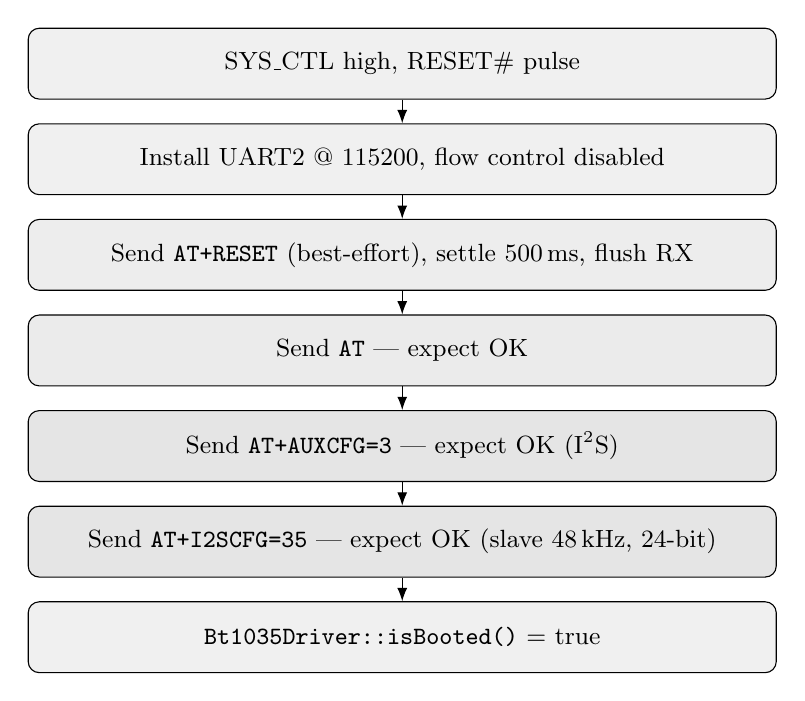
\begin{tikzpicture}[
      drstep/.style={draw, rounded corners, minimum width=9.5cm,
        minimum height=0.9cm, align=center, font=\small},
      >={Latex}, node distance=3mm]
    \node[drstep, fill=black!6] (sys) {SYS\_CTL high, RESET\# pulse};
    \node[drstep, fill=black!6, below=of sys] (uart)
      {Install UART2 @ 115200, flow control disabled};
    \node[drstep, fill=black!7, below=of uart] (swrst)
      {Send \texttt{AT+RESET} (best-effort), settle 500\,ms, flush RX};
    \node[drstep, fill=black!8, below=of swrst] (at)
      {Send \texttt{AT} --- expect OK};
    \node[drstep, fill=black!10, below=of at] (aux)
      {Send \texttt{AT+AUXCFG=3} --- expect OK (I\textsuperscript{2}S)};
    \node[drstep, fill=black!10, below=of aux] (i2s)
      {Send \texttt{AT+I2SCFG=35} --- expect OK (slave 48\,kHz, 24-bit)};
    \node[drstep, fill=black!6, below=of i2s] (done)
      {\texttt{Bt1035Driver::isBooted()} = true};
    \foreach \a/\b in {sys/uart, uart/swrst, swrst/at, at/aux, aux/i2s, i2s/done} {
      \draw[->] (\a) -- (\b);
    }
  \end{tikzpicture}
  \caption{FSC-BT1035 AT init on DigiRadio.}
  \label{fig:bt1035-boot}
\end{figure}

\begin{drnote}[AT+RESET is best-effort, not gated]
Unlike \texttt{AT+AUXCFG=3}/\texttt{AT+I2SCFG=35} (mandatory,
\texttt{core::bootInitSequence()}, boot fails if either is refused),
\texttt{AT+RESET} is sent separately and its result is discarded: it is
unverified whether this Feasycom firmware acknowledges the command before
rebooting, resets silently without a reply, or rejects it outright. Gating
boot on an unconfirmed ack would risk breaking an otherwise-working sequence.
The 500\,ms settle delay and RX flush after sending it mirror the delay
already used after the hardware GPIO reset pulse.
\end{drnote}

Pairing, codec selection, and volume over Bluetooth are handled by the
module's own firmware and NVS; DigiRadio firmware currently implements
only the I\textsuperscript{2}S bring-up required for the wired audio path.

\section{Software architecture}
\label{sec:bt1035-stack}

\begin{table}[htbp]
  \centering
  \small
  \begin{tabular}{@{}L{2.5cm}L{3.8cm}L{6.2cm}@{}}
    \drhead Layer & Type & Responsibility \\
    \midrule
    Bootstrap     & \texttt{HardwareBootstrap} &
      Constructs driver, calls \texttt{boot()} after ADAU1701 \\
    Driver        & \texttt{bt1035::Bt1035Driver} &
      UART, reset, AT init sequence \\
    Pure core     & \texttt{core::Bt1035AtCommand}, parser &
      Host-testable command strings and OK/ERROR classification \\
    \bottomrule
  \end{tabular}
  \caption{BT1035 control stack (Slice~6--7). Pairing and A2DP status are
    exposed on \texttt{/api/bluetooth/*} via \texttt{BluetoothService}.}
  \label{tab:bt1035-stack}
\end{table}

\section{Supported AT command subset}
\label{sec:bt1035-at}

The firmware enumerates every command it sends. Wire formats follow
\drpath{Hardware/DATASHEET/FSC-BT1035_programming_user_guide_1.1.1.pdf}
(§5 commands, §6 events). Extending the subset requires updating
\texttt{core::Bt1035AtCommand}, the manual, and a host test.

\begin{table}[htbp]
  \centering
  \small
  \begin{tabular}{@{}L{2.4cm}L{3.4cm}L{5.5cm}@{}}
    \drhead Enum & Line sent & Programming guide \\
    \midrule
    \texttt{Reset}          & \texttt{AT+RESET}        & software reset, best-effort \\
    \texttt{Ping}           & \texttt{AT}              & link check \\
    \texttt{I2sMode}        & \texttt{AT+AUXCFG=3}     & §5.1.25 Param=3 I2S \\
    \texttt{I2sSlave48k24}  & \texttt{AT+I2SCFG=35}    & §5.1.4 slave 48\,kHz 24-bit \\
    \texttt{PairDiscoverable} & \texttt{AT+PAIR=1} & §5.1.20 enter discoverable \\
    \texttt{PairHidden}       & \texttt{AT+PAIR=0} & §5.1.20 leave discoverable \\
    \texttt{A2dpStat}         & \texttt{AT+A2DPSTAT} & §5.3.1; states 1--5 \\
    \texttt{A2dpDisconnect}   & \texttt{AT+A2DPDISC} & §5.3.3 \\
    \texttt{QueryName}        & \texttt{AT+NAME}     & §5.1.16 read \texttt{+NAME=} \\
    \texttt{QueryAutoConn}    & \texttt{AT+AUTOCONN} & §5.1.11 read \texttt{+AUTOCONN=} \\
    \texttt{QueryPairedList}  & \texttt{AT+PLIST}    & §5.1.22; ends with \texttt{+PLIST=E} \\
    \bottomrule
  \end{tabular}
  \caption{Enumerated AT commands (\texttt{core::Bt1035AtCommand}). Boot
    sends Reset (best-effort) then the mandatory Ping + I2sMode +
    I2sSlave48k24 (\texttt{core::bootInitSequence()}); pairing commands are
    runtime.}
  \label{tab:bt1035-at}
\end{table}

Boot also calls \texttt{AT+NAME=<identity>,0} and \texttt{AT+AUTOCONN=3}
from \texttt{hardware\_bootstrap.cpp} (§5.1.16 suffix disabled, §5.1.11
reconnect count).

\section{Bt1035Driver API}
\label{sec:bt1035-driver}

\texttt{Bt1035Driver} owns UART and GPIO reset. All methods return
\texttt{std::expected<T, Bt1035Error>}.

\begin{table}[htbp]
  \centering
  \small
  \begin{tabular}{@{}L{4.2cm}L{9.2cm}@{}}
    \toprule
    \textbf{Method} & \textbf{Purpose} \\
    \midrule
    \texttt{boot()} & Reset, UART init, run \texttt{bootInitSequence()} \\
    \texttt{isBooted()} & \texttt{true} after I\textsuperscript{2}S init succeeded \\
    \texttt{sendCommand(cmd)} & Send one typed command, expect OK \\
    \texttt{enterPairingMode()} & \texttt{AT+PAIR=1} \\
    \texttt{leavePairingMode()} & \texttt{AT+PAIR=0} \\
    \texttt{queryA2dpState()} & \texttt{AT+A2DPSTAT}, parse \texttt{+A2DPSTAT=} \\
    \texttt{disconnectA2dp()} & \texttt{AT+A2DPDISC} \\
    \texttt{queryDeviceName()} & \texttt{AT+NAME}, parse \texttt{+NAME=} \\
    \texttt{queryAutoReconnect()} & \texttt{AT+AUTOCONN}, parse \texttt{+AUTOCONN=} \\
    \texttt{setAutoReconnect(times)} & \texttt{AT+AUTOCONN=n} (0--15) \\
    \texttt{queryPairedList()} & \texttt{AT+PLIST}, parse \texttt{+PLIST=} lines \\
    \bottomrule
  \end{tabular}
  \caption{Public driver API.}
  \label{tab:bt1035-api}
\end{table}

\subsection{Error codes}

\begin{table}[htbp]
  \centering
  \small
  \begin{tabular}{@{}L{4.2cm}L{9.2cm}@{}}
    \drhead \texttt{Bt1035Error} & Typical cause \\
    \midrule
    \texttt{ResetFailed}         & GPIO configuration failure \\
    \texttt{UartInitFailed}      & \texttt{uart\_driver\_install} / pins \\
    \texttt{NotBooted}           & \texttt{sendCommand} before \texttt{boot()} \\
    \texttt{AtTimeout}           & No OK/ERROR within 2\,s \\
    \texttt{AtError}             & Module returned ERROR \\
    \texttt{UnexpectedResponse}  & Unrecognised payload (future use) \\
    \bottomrule
  \end{tabular}
  \caption{Driver error enumeration.}
  \label{tab:bt1035-errors}
\end{table}

\section{Integration at power-up}
\label{sec:bt1035-integration}

\texttt{main/hardware\_bootstrap.cpp} constructs a static
\texttt{Bt1035Driver} and calls \texttt{boot()} after
\texttt{AudioService::loadAndApply()}. Failure returns
\texttt{HardwareBootError::Bt1035BootFailed} and \texttt{app\_main} halts
before network bring-up (fail-closed, same as Si4684/ADAU1701).

Boot order:
\begin{enumerate}
  \item Si4684 \texttt{boot(Dab)} --- tuner image in RAM.
  \item ADAU1701 \texttt{boot()} --- SigmaStudio program in RAM.
  \item \texttt{AudioService::loadAndApply()} --- user mixer/EQ profile.
  \item BT1035 \texttt{boot()} --- I\textsuperscript{2}S slave enabled for wireless output.
\end{enumerate}

\section{Typical usage (firmware developer)}
\label{sec:bt1035-usage}

After a successful \texttt{HardwareBootstrap::boot()}, the module is ready;
no further calls are required for basic listening. To re-send I\textsuperscript{2}S config
after a module reset:

\begin{verbatim}
bt1035::Bt1035Driver& bt = ...;
if (auto r = bt.sendCommand(core::Bt1035AtCommand::I2sMode); !r) {
  // handle Bt1035Error
}
if (auto r = bt.sendCommand(core::Bt1035AtCommand::I2sSlave48k24); !r) {
  // handle Bt1035Error
}
\end{verbatim}

\section{Further reading}
\label{sec:bt1035-reading}

\begin{itemize}
  \item \texttt{Hardware/DATASHEET/FSC-BT1035\_programming\_user\_guide\_1.1.1.pdf}
        --- authoritative AT command and event reference (§5--§6).
  \item \texttt{Hardware/DATASHEET/FSC-BT1035\_Datasheet\_EN.pdf} --- module
        electrical and pinout specification.
  \item Chapter~\ref{ch:hardware} --- pin map and I\textsuperscript{2}S routing.
  \item Chapter~\ref{ch:adau1701} --- DSP output that feeds the module.
  \item \texttt{components/core/test/bt1035\_at\_test.cpp} --- init sequence
        and parser host tests.
\end{itemize}

\chapter{HTTP API}
\label{ch:api}

The setup web interface is a thin client over a typed JSON REST API
implemented in \texttt{SetupWebServer}. Request bodies are parsed into
domain types in the pure core (\texttt{components/core}) before any
persistence or driver call. Exact C++ signatures live in the generated
Doxygen output under \texttt{docs/api/}; this chapter documents the
wire protocol and behaviour as shipped in firmware~0.9.0.

\section{Transport and reachability}

\begin{itemize}
  \item \textbf{Port:} TCP~80 on the ESP32-S3 HTTP server.
  \item \textbf{Setup mode (\texttt{NetState::SoftApSetup}):} join the
        SoftAP \texttt{DigiRadio-setup} (open network), then open
        \url{http://192.168.4.1/}. The root path serves a gzipped HTML
        page embedded from flash.
  \item \textbf{STA mode (\texttt{NetState::StaConnected}):} after
        successful provisioning and reboot, the same API is available at
        the device's DHCP address on the configured LAN.
\end{itemize}

All responses use \texttt{Content-Type: application/json} except
\texttt{GET /}, which returns gzipped HTML with
\texttt{Content-Encoding: gzip}.

\section{Endpoints}

\apiendpoint{GET}{/api/health}
\label{sec:api-health}

Returns a health-check DTO serialised by
\texttt{core::serializeHealthStatusJson()} from a
\texttt{core::HealthStatus} value.

\begin{drnote}[Response schema]
\begin{drcode}[JSON]
{"status":"ok","fw":"0.9.0","serialNumber":"0004A3123456",
 "chips":{"si4684":true,"adau1701":true,"bt1035":true}}
\end{drcode}
\begin{itemize}
  \item \texttt{status} --- coarse indicator; \texttt{ok} when the
        firmware is running normally.
  \item \texttt{fw} --- firmware release string
        (\texttt{core::FirmwareVersion}).
  \item \texttt{serialNumber} --- canonical EEPROM serial, or
        \texttt{unknown} when the 24AA025E48 read fails.
  \item \texttt{chips} --- companion-chip boot flags after
        \texttt{HardwareBootstrap::boot()} (Slice~8 integration).
\end{itemize}
\end{drnote}

HTTP status: \textbf{200 OK} on success.

\apiendpoint{POST}{/api/wifi}
\label{sec:api-wifi}

Accepts Wi-Fi credentials for station (STA) join. The body is parsed by
\texttt{core::parseWifiProvisionJson()} into a \texttt{core::WifiCredentials}
value (SSID as \texttt{core::WifiSsid}, password as \texttt{core::Secret}).
On success the credentials are persisted through
\texttt{core::ISecureStore} (device implementation:
\texttt{secure\_store::NvsSecureStore}) and the device schedules a reboot
so the next boot can enter STA mode.

\begin{drnote}[Request schema]
\begin{drcode}[JSON]
{"ssid":"MyNetwork","password":"secret1234"}
\end{drcode}
\begin{itemize}
  \item \texttt{ssid} --- required, 1--32 characters (802.11 SSID limits).
  \item \texttt{password} --- optional for open networks; for WPA-PSK,
        8--63 characters. Validated by
        \texttt{core::WifiCredentials::isPasswordValid()}.
\end{itemize}
\end{drnote}

\begin{drnote}[Success response]
\begin{drcode}[JSON]
{"status":"saved","reboot_in_sec":3}
\end{drcode}
Serialised by \texttt{core::serializeWifiProvisionSavedJson()}. The device
reboots after the indicated delay.
\end{drnote}

\begin{drnote}[Error response]
\begin{drcode}[JSON]
{"status":"error","reason":"invalid_ssid"}
\end{drcode}
Serialised by \texttt{core::serializeWifiProvisionErrorJson()}. Reason tokens (never include secrets):
\texttt{invalid\_json}, \texttt{missing\_field}, \texttt{invalid\_ssid},
\texttt{invalid\_password}, \texttt{store\_failed}.
\end{drnote}

HTTP status: \textbf{200 OK} on save success; \textbf{400 Bad Request} for
parse/validation failures; \textbf{500 Internal Server Error} when NVS
persistence fails.

\apiendpoint{POST}{/api/wifi/scan}
\label{sec:api-wifi-scan}

Lists nearby access points via \texttt{net::WifiScanner::scanNearby()} (a
blocking \texttt{esp\_wifi} scan). Empty request body.

\begin{drnote}[Response schema]
\begin{drcode}[JSON]
{"networks":[{"ssid":"MyNetwork","rssi_dbm":-52,"auth":"wpa2","channel":6}]}
\end{drcode}
Deduplicated and sorted by signal strength; \texttt{ssid} may be empty for
hidden networks.
\end{drnote}

HTTP status: \textbf{200 OK}; \textbf{500} with
\texttt{\{"status":"error","reason":"scan\_failed"\}} on driver failure.

\apiendpoint{GET}{/api/tuner/status}
\label{sec:api-tuner-status}

Returns a tuner snapshot serialised by
\texttt{core::serializeTunerStatusJson()} from \texttt{core::TunerStatus}.
The handler calls \texttt{tuner::TunerService::refreshStatus()}. DAB and FM
tuning workflows are in Chapter~\ref{ch:si4684}, Sections~\ref{sec:si4684-dab-session}
and~\ref{sec:si4684-fm-session}.

\begin{drnote}[Response schema (DAB example)]
\begin{drcode}[JSON]
{"booted":true,"band":"dab","locked":true,"volume":63,
 "dab":{"freq_index":12,"fic_quality":80,"cnr_db":25,
        "playing_service_id":42,"playing_component_id":7,
        "dynamic_label":"Live show"},
 "fm":null}
\end{drcode}
For FM, \texttt{fm} carries \texttt{frequency\_khz}, \texttt{rssi\_dbuv},
\texttt{snr\_db}, \texttt{stereo}, optional \texttt{station\_name} (RDS PS),
and \texttt{radiotext} (RDS RT); \texttt{dab} is \texttt{null}.
\end{drnote}

HTTP status: \textbf{200 OK}; \textbf{500} with
\texttt{\{"status":"error","reason":...\}} on driver failure;
\textbf{503} when the tuner service is unavailable. FM responses may include
\texttt{station\_name} and \texttt{radiotext}; DAB responses may include
\texttt{dynamic\_label} when a programme is playing.

\apiendpoint{GET}{/api/tuner/services}
\label{sec:api-tuner-services}

Lists DAB programmes for the current ensemble via
\texttt{TunerService::listDabServices()}.

\begin{drnote}[Response schema]
\begin{drcode}[JSON]
{"services":[{"service_id":12345,"component_id":1,"label":"BBC R1"}]}
\end{drcode}
\end{drnote}

HTTP status: \textbf{200 OK}; \textbf{409 Conflict} when the list cannot be
fetched (wrong band, empty ensemble, hardware error).

\apiendpoint{POST}{/api/tuner/tune}
\label{sec:api-tuner-tune}

Tunes to a DAB ensemble or FM frequency. Body parsed by
\texttt{core::parseTunerTuneJson()}.

\begin{drnote}[Request schema]
\begin{drcode}[JSON]
{"band":"dab","freq_index":12}
\end{drcode}
or
\begin{drcode}[JSON]
{"band":"fm","frequency_khz":101500}
\end{drcode}
DAB \texttt{freq\_index} is 0--37; FM \texttt{frequency\_khz} is
64\,000--108\,000. FM accepts an optional \texttt{antcap} (0--128):
overrides the front-end antenna varactor for this one tune, e.g. while
running a calibration sweep. Omit it (the normal case) to use the board's
saved calibration --- see
\texttt{POST /api/tuner/calibrate-antenna}
(Section~\ref{sec:api-tuner-calibrate-antenna}) --- or hardware auto-tune
if never calibrated. Ignored for \texttt{"dab"}.
\end{drnote}

On success returns the updated status JSON (same shape as
\texttt{GET /api/tuner/status}). HTTP status: \textbf{200 OK};
\textbf{400} for invalid JSON; \textbf{409} for tune failures.

\apiendpoint{POST}{/api/tuner/play}
\label{sec:api-tuner-play}

Starts a DAB audio service. Body parsed by
\texttt{core::parseTunerPlayJson()}.

\begin{drnote}[Request schema]
\begin{drcode}[JSON]
{"service_id":12345,"component_id":1}
\end{drcode}
\end{drnote}

Success response: \texttt{\{"status":"playing"\}}. HTTP status:
\textbf{200 OK}; \textbf{409} when playback cannot start.

\apiendpoint{POST}{/api/tuner/seek}
\label{sec:api-tuner-seek}

Seeks FM in the requested direction. Optional JSON body parsed by
\texttt{core::parseTunerSeekJson()}; an empty body defaults to upward seek.
Returns \texttt{\{"frequency\_khz":...\}} on success. HTTP status:
\textbf{200 OK}; \textbf{400} for invalid \texttt{direction}; \textbf{409} on
seek failure.

\begin{drnote}[Request schema]
\begin{drcode}[JSON]
{"direction":"up"}
\end{drcode}
Use \texttt{"down"} for downward seek. Omit the body or send an empty JSON
object (\texttt{\{\}}) for upward seek (backward compatible).
\end{drnote}

\apiendpoint{POST}{/api/tuner/scan}
\label{sec:api-tuner-scan}

Automatic search for a single station: repeats hardware seeks (FM) or
walks ensemble indices (DAB) via \texttt{TunerService::scanForStation()},
stopping early on the first usable hit, optionally filtered by name. This
blocks the HTTP connection for the whole search (up to tens of seconds).

\begin{drnote}[Request schema]
\begin{drcode}[JSON]
{"band":"fm","max_steps":45,"name":"BBC"}
\end{drcode}
\texttt{band} is required (\texttt{"fm"} or \texttt{"dab"}).
\texttt{max\_steps} is optional, 1--255 (default 45 for FM, 38 for DAB).
\texttt{name} is an optional case-insensitive substring match against the
RDS PS name (FM) or DAB service label.
\end{drnote}

\begin{drnote}[Response schema]
\begin{drcode}[JSON]
{"status":"found","band":"fm","steps":12,"frequency_khz":97500,
 "station_name":"BBC R1"}
\end{drcode}
\texttt{status} is \texttt{"found"} or \texttt{"not\_found"}. On a DAB hit,
\texttt{freq\_index}, \texttt{service\_id}, and \texttt{component\_id}
appear instead of \texttt{frequency\_khz}.
\end{drnote}

HTTP status: \textbf{200 OK} (including \texttt{"not\_found"} outcomes);
\textbf{400} for invalid JSON; \textbf{409} on a hardware/driver failure
mid-scan.

\apiendpoint{POST}{/api/tuner/scan/full}
\label{sec:api-tuner-scan-full}

Sweeps the entire FM band with repeated hardware seeks
(\texttt{TunerService::scanFullFmBand()}) and returns every usable station
found, in ascending frequency order. Does \emph{not} save results as
presets --- this only returns the list; use
\texttt{POST /api/stations} (Section~\ref{sec:api-stations-post}) to save
individual hits. Empty request body; blocks for the whole sweep (tens of
seconds).

\begin{drnote}[Response schema]
\begin{drcode}[JSON]
{"stations":[{"frequency_khz":97500,"rssi_dbuv":58,"snr_db":21,
              "station_name":"BBC R1"},
             {"frequency_khz":101500,"rssi_dbuv":44,"snr_db":15}]}
\end{drcode}
\texttt{station\_name} (RDS PS) is present only when decoded before the
per-station poll budget ran out.
\end{drnote}

HTTP status: \textbf{200 OK}; \textbf{409} on a hardware/driver failure
mid-sweep; \textbf{503} when the tuner service is unavailable.

\apiendpoint{POST}{/api/tuner/calibrate-antenna}
\label{sec:api-tuner-calibrate-antenna}

Commits an FM ANTCAP value (AN851 Appendix A front-end calibration) as the
board's permanent default, found by sweeping \texttt{antcap} on
\texttt{POST /api/tuner/tune} (Section~\ref{sec:api-tuner-tune}) across
0--128 and comparing \texttt{rssi\_dbuv}/\texttt{snr\_db}. Persists to the
24AA025E48 EEPROM's user-writable region (separate from the factory-locked
EUI-48) and takes effect immediately on the live tuner --- no reboot
required, though it also survives one since \texttt{HardwareBootstrap::boot()}
reloads it at every boot. Once saved, every ordinary FM tune (seek, scan,
station recall, live UI) uses this value automatically instead of the
chip's own front-end auto-tune, unless a request explicitly overrides
\texttt{antcap} for that one call.

\begin{drnote}[Request schema]
\begin{drcode}[JSON]
{"antcap":102}
\end{drcode}
\texttt{antcap} is required, 0--128.
\end{drnote}

Success response: \texttt{\{"status":"saved","antcap":102\}}. HTTP status:
\textbf{200 OK}; \textbf{400} for invalid/missing \texttt{antcap};
\textbf{500} on an EEPROM write failure; \textbf{503} when the tuner
service is unavailable.

\apiendpoint{GET}{/api/audio/profile}
\label{sec:api-audio-profile-get}

Returns the current ADAU1701 audio snapshot serialised by
\texttt{core::serializeAudioProfileJson()} from \texttt{core::AudioProfile}.
The handler reads \texttt{audio::AudioService::currentProfile()}. Driver
behaviour, domain types, and persistence are documented in
Chapter~\ref{ch:adau1701}.

\begin{drnote}[Response schema (excerpt)]
\begin{drcode}[JSON]
{"mixer":{"si4684_left_db":0,"si4684_right_db":0,
         "esp32_left_db":0,"esp32_right_db":0,
         "mix_left_db":0,"mix_right_db":0},
 "master":{"left_db":0,"right_db":0},
 "eq":[{"gain_db":0,"center_hz":40,"q":1.414}, ...],
 "enhancements":{"stereo_level":0,"bass_level":0}}
\end{drcode}
Six EQ bands are always present (\texttt{eq} array length~6).
Enhancement levels are 0--100; at 0 the base EQ band settings apply.
\end{drnote}

HTTP status: \textbf{200 OK}; \textbf{503} when the audio service is
unavailable.

\apiendpoint{PUT}{/api/audio/profile}
\label{sec:api-audio-profile-put}

Applies a full audio profile. Body parsed by
\texttt{core::parseAudioProfileJson()}; on success
\texttt{audio::AudioService::applyProfile(..., persist=true)} safeloads
the ADAU1701 and writes NVS key \texttt{audio\_profile\_json}.

\begin{drnote}[Success response]
\begin{drcode}[JSON]
{"status":"saved"}
\end{drcode}
\end{drnote}

HTTP status: \textbf{200 OK}; \textbf{400} for parse/validation failures;
\textbf{500} when safeload or NVS persistence fails.

\apiendpoint{POST}{/api/dsp/program}
\label{sec:api-dsp-program}

Uploads a framed ADAU1701 RAM download blob (\texttt{DRAD} v1, see
\texttt{core::parseDspProgramBlob()}). The body is raw bytes
(\texttt{application/octet-stream} or any content type). On success the blob
is written to the \texttt{dsp} flash partition and the device reboots; the
next boot replays the new program before \texttt{loadAndApply()}.

\begin{drnote}[Success response]
\begin{drcode}[JSON]
{"status":"stored","reboot_sec":3}
\end{drcode}
\end{drnote}

HTTP status: \textbf{200 OK}; \textbf{400} with \texttt{\{"error":"..."\}}
for invalid/truncated/CRC failures; \textbf{413} when the body exceeds
200\,KiB; \textbf{500} on flash write failure. Pack blobs with
\texttt{tools/pack\_dsp\_program.py} or \texttt{core::serializeDspProgramBlob()}.

\apiendpoint{POST}{/api/system/ota}
\label{sec:api-system-ota}

Streams a raw ESP-IDF application \texttt{.bin} into the inactive OTA slot
(\texttt{ota\_0}/\texttt{ota\_1}). The body is raw bytes; the server validates
the embedded \texttt{esp\_app\_desc\_t} at offset~0x20 (magic and
\texttt{project\_name == "digiradio"}) while streaming. On success the new
slot is selected and the device reboots; the first healthy boot after Wi-Fi
and HTTP are up calls
\texttt{ota::OtaService::confirmBoot()} to cancel rollback.

\begin{drnote}[Success response]
\begin{drcode}[JSON]
{"status":"stored","reboot_sec":3}
\end{drcode}
\end{drnote}

HTTP status: \textbf{200 OK}; \textbf{400} with \texttt{\{"error":"..."\}}
for invalid project/magic or flash write failures;
\textbf{413} when the body exceeds 1.7\,MiB (\texttt{0x1B0000});
\textbf{500} on \texttt{esp\_ota\_end}/set-boot failures. Push with
\texttt{curl --data-binary @build/digiradio.bin}.

\apiendpoint{POST}{/api/audio/reset}
\label{sec:api-audio-reset}

Restores \texttt{AudioProfile::factoryDefault()} (flat EQ, 0\,dB gains),
applies it to the DSP, and persists to NVS. Success response:
\texttt{\{"status":"saved"\}}. HTTP status: \textbf{200 OK}; \textbf{500}
on apply/persist failure.

\apiendpoint{POST}{/api/audio/stereo-enhance}
\label{sec:api-audio-stereo-enhance}

Adjusts stereo depth via a psychoacoustic PEQ overlay on bands 3--5
(1\,kHz / 3\,kHz / 8\,kHz). This is \emph{not} true M/S widening---there
is no dedicated SigmaStudio widener block; see
Section~\ref{sec:ss-enhancements}.

\begin{drnote}[Request body]
\begin{drcode}[JSON]
{"level":50}
\end{drcode}
\texttt{level} is an integer 0--100 (0 = off, 100 = maximum).
\end{drnote}

Success response: \texttt{\{"status":"saved"\}}. HTTP status:
\textbf{200 OK}; \textbf{400} for invalid JSON or level; \textbf{500}
when safeload or NVS persistence fails.

\apiendpoint{POST}{/api/audio/bass-enhance}
\label{sec:api-audio-bass-enhance}

Adjusts bass emphasis via a PEQ overlay on bands 1--2 (100\,Hz /
400\,Hz). Request and response schema match
\texttt{POST /api/audio/stereo-enhance} (Section~\ref{sec:api-audio-stereo-enhance}).

\apiendpoint{POST}{/api/audio/beep}
\label{sec:api-audio-beep}

Toggles the ADAU1701's own Beep1 tone generator cell directly (live
safeload only --- not part of \texttt{AudioProfile}, never persisted to
NVS). Used for signal-path bring-up/diagnostics without an ESP32-side
tone source.

\begin{drnote}[Request schema]
\begin{drcode}[JSON]
{"enabled":true}
\end{drcode}
\end{drnote}

Success response: \texttt{\{"status":"saved"\}}. HTTP status:
\textbf{200 OK}; \textbf{400} for invalid/missing \texttt{enabled};
\textbf{500} on safeload failure; \textbf{503} when the audio service is
unavailable.

\apiendpoint{GET}{/api/dsp/params}
\label{sec:api-dsp-params}

Lists every named Parameter RAM cell in the compiled SigmaStudio program
(\texttt{adau1701::kAdau1701ParamTable}, generated from
\texttt{DigiRadio\_IC\_1\_PARAM.h}). Read-only, no I/O with the chip.

\begin{drnote}[Response schema (excerpt)]
\begin{drcode}[JSON]
{"params":[{"name":"DspGain1algorithm0dB1","address":0},
           {"name":"Beep1osc1algorithm0freq","address":16}]}
\end{drcode}
\end{drnote}

HTTP status: \textbf{200 OK}.

\apiendpoint{PUT}{/api/dsp/param}
\label{sec:api-dsp-param}

Writes one Parameter RAM cell by name, looked up against the same table as
\texttt{GET /api/dsp/params} and safeloaded via
\texttt{audio::AudioService::writeRawParam()}. This is a live-only escape
hatch onto \emph{any} SigmaStudio-exported cell --- the same trust level as
SigmaStudio's own Remote Connection panel: no domain validation on the
value, and it is never persisted or folded into \texttt{AudioProfile}. A
reboot or \texttt{POST /api/audio/reset} discards the change.

\begin{drnote}[Request schema]
\begin{drcode}[JSON]
{"name":"DspGain1algorithm0dB1","value":-6.0}
\end{drcode}
\texttt{value} is the SigmaStudio floating coefficient, converted to
8.23 fixed-point by \texttt{core::floatToFixpoint823()} before the
safeload write.
\end{drnote}

Success response: \texttt{\{"status":"saved"\}}. HTTP status:
\textbf{200 OK}; \textbf{400} for invalid JSON; \textbf{404} when
\texttt{name} is not in the compiled program's cell table; \textbf{500}
on safeload failure; \textbf{503} when the audio service is unavailable.

\apiendpoint{PUT}{/api/stream/phone}
\label{sec:api-stream-phone}

Accepts a live audio push from a phone app and writes it straight to the
shared I2S sink for as long as the connection stays open --- the same
physical wire \texttt{POST /api/streaming}'s web radio player uses, guarded
so only one producer holds it at a time. The body is raw interleaved
16-bit little-endian PCM, stereo, 48\,kHz, with \emph{no} header or
framing --- just samples. Send with chunked transfer encoding (no
\texttt{Content-Length} required) and close the connection to stop
streaming; the format is deliberately unencoded so the firmware side stays
minimal and the encoding choice lives entirely in the app.

HTTP status: \textbf{503} if the sink is unavailable; \textbf{409 Conflict}
if the web radio stream (or another phone stream) currently owns the I2S
sink; otherwise the connection is held open and a \textbf{200 OK} (empty
body) is sent once the client closes it, or \textbf{500} if a write to the
sink fails mid-stream.

\apiendpoint{GET}{/api/streaming}
\label{sec:api-streaming-get}

Returns the current internet radio streaming configuration
(\texttt{webradio::WebRadioService::config()}).

\begin{drnote}[Response schema]
\begin{drcode}[JSON]
{"enabled":true,"url":"http://stream.example.com/radio.mp3"}
\end{drcode}
\end{drnote}

HTTP status: \textbf{200 OK}; \textbf{503} when the web radio service is
unavailable.

\apiendpoint{POST}{/api/streaming}
\label{sec:api-streaming-post}

Sets the internet radio stream URL and enables/disables playback. Applied
immediately to the live streaming task and persisted to NVS --- no reboot
required. The stream is MP3 over HTTP, decoded on-device via libhelix and
written to the same shared I2S sink as \texttt{PUT /api/stream/phone}.

\begin{drnote}[Request schema]
\begin{drcode}[JSON]
{"enabled":true,"url":"http://stream.example.com/radio.mp3"}
\end{drcode}
\texttt{url} must be \texttt{http://}, non-empty, and at most 200 bytes.
\end{drnote}

On success, returns the same shape as \texttt{GET /api/streaming}. HTTP
status: \textbf{200 OK}; \textbf{400} for invalid JSON or URL;
\textbf{500} when NVS persistence fails; \textbf{503} when the web radio
service is unavailable.

% ------------------------------------------------------------------
% Bluetooth (Slice 7)
% ------------------------------------------------------------------

\apiendpoint{GET}{/api/bluetooth/status}
\label{sec:api-bluetooth-status}

Returns BT1035 boot flag, whether discoverable mode was requested, the
last read A2DP state, module friendly name, and auto-reconnect count.
Serialised by \texttt{core::serializeBluetoothStatusJson()}.

\begin{drnote}[Response schema]
\begin{drcode}[JSON]
{"booted":true,"pairing":false,"a2dp":"standby",
 "device_name":"DigiRadio-A1B2","auto_reconnect":3}
\end{drcode}
\end{drnote}

\apiendpoint{POST}{/api/bluetooth/pair}
\label{sec:api-bluetooth-pair}

Enters discoverable mode (\texttt{AT+PAIR=1}). Success:
\texttt{\{"status":"pairing"\}}.

\apiendpoint{POST}{/api/bluetooth/pair/stop}
\label{sec:api-bluetooth-pair-stop}

Leaves discoverable mode (\texttt{AT+PAIR=0}). Success:
\texttt{\{"status":"idle"\}}.

\apiendpoint{POST}{/api/bluetooth/disconnect}
\label{sec:api-bluetooth-disconnect}

Releases the current A2DP session (\texttt{AT+A2DPDISC}).

\apiendpoint{GET}{/api/bluetooth/paired}
\label{sec:api-bluetooth-paired}

Returns paired remotes from \texttt{AT+PLIST}, serialised by
\texttt{core::serializeBluetoothPairedJson()}.

\begin{drnote}[Response schema]
\begin{drcode}[JSON]
{"devices":[{"index":1,"mac":"001122334455","name":"Phone"}]}
\end{drcode}
\end{drnote}

\apiendpoint{POST}{/api/bluetooth/scan}
\label{sec:api-bluetooth-scan}

Scans for nearby Bluetooth devices via \texttt{AT+DISC} on the BT1035
(\texttt{bluetooth::BluetoothService::scanNearby()}). Blocks for the scan
window.

\begin{drnote}[Request schema]
\begin{drcode}[JSON]
{"seconds":45}
\end{drcode}
\texttt{seconds} is optional, 1--255 (default 45); malformed or
out-of-range values fall back to the default rather than failing.
\end{drnote}

\begin{drnote}[Response schema]
\begin{drcode}[JSON]
{"devices":[{"index":1,"mac":"001122334455","name":"Bose SoundLink",
             "rssi_dbm":-58}]}
\end{drcode}
\end{drnote}

HTTP status: \textbf{200 OK}; \textbf{500} on a BT1035 driver error;
\textbf{503} when the Bluetooth service is unavailable.

\apiendpoint{POST}{/api/bluetooth/connect}
\label{sec:api-bluetooth-connect}

Connects A2DP to a specific remote MAC, optionally saving it as the
default speaker for auto-reconnect on boot
(\texttt{BluetoothService::connectTo()}).

\begin{drnote}[Request schema]
\begin{drcode}[JSON]
{"mac":"001122334455","name":"Bose SoundLink","save":true}
\end{drcode}
\texttt{mac} is required (12 hex characters, no separators). \texttt{name}
and \texttt{save} are optional; when \texttt{save} is true, \texttt{mac}
and \texttt{name} are persisted the same way as
\texttt{POST /api/bluetooth/speaker}.
\end{drnote}

Success response: \texttt{\{"status":"connected"\}}. HTTP status:
\textbf{200 OK}; \textbf{400} when \texttt{mac} is missing/invalid;
\textbf{500} on a BT1035 driver error; \textbf{503} when the Bluetooth
service is unavailable.

\apiendpoint{GET}{/api/bluetooth/speaker}
\label{sec:api-bluetooth-speaker-get}

Returns the saved default-speaker target used for boot-time auto-reconnect,
if any.

\begin{drnote}[Response schema]
\begin{drcode}[JSON]
{"configured":true,"mac":"001122334455","name":"Bose SoundLink"}
\end{drcode}
\texttt{\{"configured":false\}} when nothing is saved.
\end{drnote}

HTTP status: \textbf{200 OK}; \textbf{500} on an NVS read failure;
\textbf{503} when the Bluetooth service is unavailable.

\apiendpoint{POST}{/api/bluetooth/speaker}
\label{sec:api-bluetooth-speaker-post}

Saves (or replaces) the default-speaker target, without connecting
immediately. Request schema matches
\texttt{POST /api/bluetooth/connect} minus \texttt{save} (\texttt{mac}
required, \texttt{name} optional).

Success response: \texttt{\{"status":"saved"\}}. HTTP status:
\textbf{200 OK}; \textbf{400} for invalid JSON; \textbf{500} on an NVS
write failure; \textbf{503} when the Bluetooth service is unavailable.

\apiendpoint{DELETE}{/api/bluetooth/speaker}
\label{sec:api-bluetooth-speaker-delete}

Clears the saved default-speaker target; boot-time auto-reconnect is
skipped until a new one is saved. Success response:
\texttt{\{"status":"cleared"\}}. HTTP status: \textbf{200 OK};
\textbf{503} when the Bluetooth service is unavailable.

\apiendpoint{POST}{/api/bluetooth/reconnect}
\label{sec:api-bluetooth-reconnect}

Manually retries A2DP connect to the saved default speaker
(\texttt{BluetoothService::reconnectSavedSpeaker()}) --- the same call the
firmware makes once at boot. Empty request body.

Success response: \texttt{\{"status":"connected"\}}. HTTP status:
\textbf{200 OK}; \textbf{500} on a BT1035 driver error or when no speaker
is saved; \textbf{503} when the Bluetooth service is unavailable.

\apiendpoint{POST}{/api/bluetooth/auto-reconnect}
\label{sec:api-bluetooth-auto-reconnect}

Sets the module auto-reconnect retry count (\texttt{AT+AUTOCONN=0..15}).
Body parsed by \texttt{core::parseBluetoothAutoReconnectJson()}.

\begin{drnote}[Request schema]
\begin{drcode}[JSON]
{"times":3}
\end{drcode}
Success: \texttt{\{"status":"saved"\}}.
\end{drnote}

% ------------------------------------------------------------------
% Station presets (Slice 4)
% ------------------------------------------------------------------

\apiendpoint{GET}{/api/stations}
\label{sec:api-stations-get}

Returns presets serialised by \texttt{core::serializeStationListJson()}.

\apiendpoint{POST}{/api/stations}
\label{sec:api-stations-post}

Adds one preset (\texttt{core::parseStationJson()}); persists via
\texttt{ISecureStore::saveStationListJson()}.

\apiendpoint{POST}{/api/stations/remove}
\label{sec:api-stations-remove}

Removes a preset by list index (\texttt{\{"index":0\}}).

\apiendpoint{POST}{/api/stations/reorder}
\label{sec:api-stations-reorder}

Reorders presets using \texttt{StationList::move()}. Body:
\texttt{\{"from":1,"to":0\}}. Success: \texttt{\{"status":"reordered"\}}.

\apiendpoint{POST}{/api/stations/tune}
\label{sec:api-stations-tune}

Recalls a preset via \texttt{integration::IntegrationService::recallPreset()}
(tune, re-apply saved audio profile, persist last index).

\section{Boot and network state machine}
\label{sec:api-boot-flow}

At boot, \texttt{integration::IntegrationService::startup()} loads presets
and best-effort recalls the last station. Then
\texttt{net::NetBootstrap::start(store, tuner, audio, bluetooth, stations,
integration)} consults \texttt{ISecureStore::hasWifiCredentials()}:

\begin{enumerate}
  \item \textbf{Credentials present} --- create STA netif, connect via
        \texttt{net::StaClient} (30\,s timeout). On success:
        \texttt{NetState::StaConnected} and HTTP on the LAN address.
  \item \textbf{No credentials, or STA join fails} --- fall back to
        SoftAP setup mode (\texttt{NetState::SoftApSetup}).
\end{enumerate}

This explicit \texttt{enum class NetState} replaces ad-hoc flags; see
\texttt{net/NetState.hpp} in the source tree.

\subsection{BLE provisioning (additive)}
\label{sec:api-boot-ble-provisioning}

Alongside the SoftAP, setup mode also starts ESP-IDF's own
\texttt{wifi\_provisioning} manager over BLE
(\texttt{net::ble\_provisioning::start()}), using the ESP32-S3's onboard
BLE radio --- independent of the BT1035, which stays a separate UART-attached
classic-Bluetooth A2DP module. This is the standard Espressif provisioning
protocol (protocomm, Security1), so any generic ``ESP BLE Provisioning''
app (iOS/Android) can join the device to Wi-Fi without first connecting to
\texttt{DigiRadio-setup}; the proof-of-possession string is the device's
own serial number (same source as the SoftAP SSID and
\texttt{GET /api/health}'s \texttt{serialNumber}). It is not an HTTP
endpoint --- there is no REST call here --- and it is strictly additive:
if it fails to start, SoftAP setup keeps working exactly as before. On a
successful join the received credentials are converted to the same
\texttt{core::WifiCredentials} type and saved through the same
\texttt{ISecureStore} that \texttt{POST /api/wifi} uses, then the device
reboots into STA mode.

\section{Credential storage (Slice~2)}
\label{sec:api-storage}

Wi-Fi credentials are stored in NVS namespace \texttt{digiradio}, keys
\texttt{wifi\_ssid} and \texttt{wifi\_pwd}. Audio profiles (non-secret) use
the same namespace, key \texttt{audio\_profile\_json}, via
\texttt{secure\_store::NvsAudioProfileStore}. Station presets use key
\texttt{station\_list} (JSON blob). The last recalled preset index is stored
as \texttt{last\_preset} (u8). Passwords are wrapped in
\texttt{core::Secret} in RAM and are never logged or returned by the API.

\begin{drcaution}[Encryption at rest]
Firmware~0.8.3+ enables NVS encryption
(\texttt{CONFIG\_NVS\_ENCRYPTION}) and flash encryption in development mode
(\texttt{sdkconfig.defaults}). Keys live in the \texttt{nvs\_keys} partition;
Wi-Fi passwords remain wrapped in \texttt{core::Secret} in RAM and are never
logged. First upgrade from plain NVS requires \texttt{idf.py erase-flash}.
HIL checklist: \drpath{Software/docs/security-flash-nvs.md}.
\end{drcaution}

\chapter{Class Reference}
\label{ch:classes}

This chapter documents the firmware's public classes at the design level:
what each class is responsible for, which collaborators it depends on, its
key invariants, and how it fits the system. It complements --- and does
not duplicate --- the generated API documentation, which carries the exact
method signatures. The HTTP JSON endpoints are documented separately in
Chapter~\ref{ch:api}.

\begin{drnote}[How this chapter grows]
Per the development rules, every public, architecturally-significant class
(the drivers, the application services, and the public domain-core types)
gets a section here, tagged \texttt{\textbackslash label\{cls:ClassName\}},
added in the same change that introduces the class. A tooling check keeps
this chapter in step with the code, so it is always current.
\end{drnote}

The firmware is under active development. As each public class lands, its
section appears below, grouped by layer: domain core, application
services, and hardware drivers.

% ------------------------------------------------------------------
% Domain core (Slice 1)
% ------------------------------------------------------------------

\section{FirmwareVersion}\label{cls:FirmwareVersion}
Strong type wrapping the firmware release identifier (e.g.\ \texttt{0.1.0}).
Used by \texttt{HealthStatus} and the \texttt{/api/health} endpoint so
version strings are never passed as bare \texttt{char*} across module
boundaries. Invariant: non-empty at construction.

\section{HealthStatus}\label{cls:HealthStatus}
Immutable health-check DTO returned by \texttt{GET /api/health}. Built via
\texttt{HealthStatus::ok(FirmwareVersion)} in the pure core; JSON
serialisation lives in \texttt{serializeHealthStatusJson()}. No ESP-IDF
headers.

% ------------------------------------------------------------------
% Network shell (Slice 1)
% ------------------------------------------------------------------

\section{SoftApConfig}\label{cls:SoftApConfig}
Immutable value type holding SoftAP parameters (SSID, channel, station
limit). Factory \texttt{setupDefault()} yields SSID \texttt{DigiRadio-setup}
for first-time provisioning.

\section{SoftApHost}\label{cls:SoftApHost}
RAII wrapper around the ESP-IDF Wi-Fi stack that starts and stops the
configured SoftAP. Imperative shell; no business logic.

\section{SetupWebServer}\label{cls:SetupWebServer}
Minimal HTTP server: gzipped setup UI, \texttt{GET /api/health},
\texttt{POST /api/wifi}, and tuner routes (\texttt{/api/tuner/*}).
JSON parsing and serialisation delegate to the pure core; credentials
persist via \texttt{ISecureStore}; tuner operations via
\texttt{tuner::TunerService}.

\section{NetBootstrap}\label{cls:NetBootstrap}
Owns network resources for setup or STA mode.
\texttt{start(store, tuner)} initialises the platform, joins stored Wi-Fi
when credentials exist, or falls back to the \texttt{DigiRadio-setup}
SoftAP. Must outlive \texttt{app\_main} for the process lifetime.

% ------------------------------------------------------------------
% Domain core + secure store (Slice 2)
% ------------------------------------------------------------------

\section{Secret}\label{cls:Secret}
Opaque wrapper for sensitive strings. Buffer is zeroised on destruction;
no \texttt{operator<<} and no plaintext serialisation. Shell code uses
\texttt{usePlaintext()} transiently for driver APIs only.

\section{WifiSsid}\label{cls:WifiSsid}
Validated Wi-Fi SSID (1--32 bytes). Parsed once from untrusted JSON at
the HTTP boundary before persistence or driver calls.

\section{WifiCredentials}\label{cls:WifiCredentials}
Domain value pairing \texttt{WifiSsid} with a \texttt{Secret} password.
Open networks use an empty password; WPA-PSK requires 8--63 characters.

\section{ISecureStore}\label{cls:ISecureStore}
Abstract persistence boundary for credentials at rest. Slice~2 implements
Wi-Fi credential save/load/clear; station list and user credentials arrive
in later slices. Host tests use fakes; the shell uses \texttt{NvsSecureStore}.

\section{StaClient}\label{cls:StaClient}
RAII STA join helper with an explicit connect timeout. Assumes
\texttt{esp\_wifi\_init()} was already called by \texttt{NetBootstrap}.

\section{NvsSecureStore}\label{cls:NvsSecureStore}
\texttt{ISecureStore} implementation backed by an NVS namespace. Passwords
are stored as NVS strings and never logged. Production should enable NVS
encryption using the reserved \texttt{nvs\_keys} partition.

% ------------------------------------------------------------------
% Hardware drivers (Slice 3)
% ------------------------------------------------------------------

\section{IFirmwareBlobReader}\label{cls:IFirmwareBlobReader}
Abstract streaming reader for firmware blobs embedded in flash. The Si4684
driver uses it to HOST\_LOAD patch and application images in bounded SPI
chunks without allocating the full image on the heap. Host tests use the
same interface over in-memory buffers.

\section{EmbeddedBlobReader}\label{cls:EmbeddedBlobReader}
Non-owning \texttt{IFirmwareBlobReader} over a contiguous byte range (linker
symbols from \texttt{EMBED\_FILES} or test data). Implements offset-based
\texttt{read()} with truncation at end-of-blob.

\section{Si4684EmbeddedImages}\label{cls:Si4684EmbeddedImages}
Owns \texttt{EmbeddedBlobReader} views over \texttt{rom\_patch\_016.bin},
\texttt{dab\_firmware.bin}, and \texttt{fm\_firmware.bin}. Constructed once;
passed to \texttt{Si4684Driver}. \texttt{applicationImage(Si4684Band)} selects
DAB or FM.

\section{Si4684Driver}\label{cls:Si4684Driver}
Full SPI driver for the Si4684 DAB+/FM tuner (Chapter~\ref{ch:si4684}).

\texttt{boot(Si4684Band)} runs AN649 HOST\_LOAD, configures I\textsuperscript{2}S
and band-specific properties, and records \texttt{loadedBand()}. After boot the
driver exposes FM tuning/seek/RSQ/RDS, DAB ensemble tuning, digital service list
fetch, and \texttt{startDabService}. Property access (\texttt{setProperty},
\texttt{setVolume}) and diagnostics (\texttt{getPartInfo}, \texttt{getSysState})
are included. Wrong-band calls return \texttt{Si4684Error::WrongBand}.
Register-level opcodes remain private; see \texttt{Si4684Types.hpp} for status
DTOs.

\section{Adau1701Driver}\label{cls:Adau1701Driver}
RAII I2C driver for the ADAU1701 SigmaDSP. \texttt{boot()} asserts RESET\#,
initialises the shared I2C bus, and replays the SigmaStudio export from
\texttt{Firmware/ADAU1701-Firmware/} on every power-up (no EEPROM self-boot
on DigiRadio).

% ------------------------------------------------------------------
% Application services (Slice 4)
% ------------------------------------------------------------------

\section{ITuner}\label{cls:ITuner}
Abstract tuner boundary in the pure core. Defines boot, band selection,
status readout, FM/DAB tuning, service list, playback, and volume without
ESP-IDF types. \texttt{si4684::Si4684Tuner} implements it on device; host
tests can use fakes.

\section{TunerService}\label{cls:TunerService}
Application service exposing intent-level tuner operations to HTTP and
future UI. Holds a reference to \texttt{core::ITuner}, tracks last tune
target and volume, and maps driver failures to \texttt{core::TunerError}.

\section{Si4684Tuner}\label{cls:Si4684Tuner}
\texttt{ITuner} adapter over \texttt{Si4684Driver}. Translates domain calls
into SPI commands and maps \texttt{Si4684Error} to \texttt{TunerError}.
Constructed once in \texttt{HardwareBootstrap} alongside the driver.

\chapter{Building and Flashing}
\label{ch:build}

The firmware is built with ESP-IDF; the hardware-free domain core also
builds and is unit-tested on the host machine.

\section{Toolchain}

\begin{table}[htbp]
  \centering
  \begin{tabular}{@{}ll@{}}
    \drhead Item & Choice \\
    \midrule
    Framework        & ESP-IDF v5.5.x (native) \\
    Language          & C++23 (\texttt{-std=gnu++23}) \\
    Error model       & \texttt{std::expected}; exceptions off \\
    Documentation     & Doxygen (build must pass) \\
    \bottomrule
  \end{tabular}
  \caption{Firmware toolchain.}
  \label{tab:build-toolchain}
\end{table}

\section{Device build}

\begin{drcode}[Build, flash, monitor]
idf.py set-target esp32s3
idf.py build
idf.py -p <port> flash monitor
\end{drcode}

\section{Host unit tests}

The pure core is tested on the host, with no board attached. On macOS the
tests need a C++23 standard library --- use a Homebrew LLVM (>= 18) or
GCC~14 rather than the system Apple Clang.

\begin{drcode}[Host tests]
cmake -S components/core/test -B build-host \
      -DCMAKE_CXX_COMPILER="$(brew --prefix llvm)/bin/clang++"
cmake --build build-host
ctest --test-dir build-host --output-on-failure
\end{drcode}

\section{Documentation}

Documentation has two enforced checks, run from the \texttt{Software/}
directory:

\begin{enumerate}
  \item \textbf{Doxygen} --- C++ API reference from source doc blocks.
        An undocumented public class, method, or parameter fails the build.
  \item \textbf{Manual sync} --- every public class under an
        \texttt{include/} tree must have a matching
        \texttt{\textbackslash label\{cls:ClassName\}} section in
        \texttt{docs/manual/ch-classes.tex}. Design-level HTTP API
        documentation lives in Chapter~\ref{ch:api}.
\end{enumerate}

\begin{drcode}[Docs (from Software/)]
doxygen Doxyfile
python3 tools/check-manual-sync.py
\end{drcode}

To rebuild the PDF manual (requires a LaTeX installation):

\begin{drcode}[Manual PDF]
cd docs/manual
latexmk -lualatex manual.tex
\end{drcode}

\begin{drcaution}[Keep it green]
Both checks are part of the definition of done. A firmware change that
adds or modifies a public class, a REST endpoint, or its behaviour must
update the Doxygen doc blocks, \texttt{ch-classes.tex} (for classes), and
\texttt{ch-api.tex} (for HTTP) in the same change.
\end{drcaution}

\chapter{Licensing}
\label{ch:licensing}

DigiRadio is dual-licensed, with hardware and firmware under separate but
compatible open-source licences.

\section{Hardware}

The hardware --- schematics, PCB layout, Gerbers, and bill of materials
--- is licensed under the \textbf{CERN Open Hardware Licence Version~2,
Strongly Reciprocal (CERN-OHL-S v2)}. Anyone who modifies and distributes
the hardware must release their changes under the same terms.

\section{Firmware}

The firmware is licensed under the \textbf{Apache License 2.0}. It grants
patent rights explicitly and pairs naturally with the ESP-IDF ecosystem,
which is Apache-licensed as well. Every source file carries the Apache
header with an SPDX identifier.

\section{Documentation and project pages}

Where a hosting platform does not offer the CERN-OHL-S licence in its
selector, the closest share-alike option is used for that page, with the
authoritative licence stated as CERN-OHL-S v2. The definitive licensing
is always the one declared in the project repository.

\section{Third-party components}

The design integrates third-party silicon (Silicon Labs, Analog Devices,
Espressif, Feasycom/Qualcomm) whose datasheets, firmware images, and DSP
tools remain subject to their respective vendors' terms. Those terms are
unaffected by the DigiRadio licences and must be observed when
redistributing vendor-supplied binaries.

\begin{drnote}[Manufacturing partner]
Prototype fabrication and assembly are supported by PCBWay. Their
contribution is acknowledged in the project documentation and on the
board.
\end{drnote}


% ---------------- Back cover (acknowledgements) ----------------
\cleardoublepage
\thispagestyle{empty}
\vspace*{\fill}
\begin{center}
{\color{drPetrol}\Large\bfseries Acknowledgements\par}
\vspace{1.2cm}
\begin{minipage}{0.82\textwidth}
\centering
{\color{drInk}
\textbf{PCBWay} sponsored part of the prototype PCB fabrication and assembly
costs for DigiRadio. Their contribution did not cover the full production
budget, but it materially reduced the out-of-pocket expense of the first
manufacturing run. We thank the PCBWay team for believing in this open hardware
project and for helping bring the first boards to life.\par}
\vspace{1.2cm}

\includegraphics[width=0.32\textwidth]{figures/pcbway-logo.png}%
\vspace{0.8cm}
{\color{drGray}\small\url{https://www.pcbway.com}\par}
\end{minipage}
\end{center}
\vspace*{\fill}

\end{document}
